\documentclass[a4paper,11pt,twoside,openright]{book} % Type du document

% compiler avec : pdflatex, bibtex, pdflatex, pdflatex


% +---------------------------------------------------------------+
% | Language
% +---------------------------------------------------------------+
\usepackage[T1]{fontenc}
\usepackage[utf8]{inputenc}
\usepackage[french]{babel}
\usepackage{url}
\usepackage{pgf-umlsd}
\usepackage{adjustbox}
\raggedbottom


\newif\ifisconfidential	\isconfidentialfalse

\newif\ifisdraft\isdraftfalse



% +---------------------------------------------------------------+
% | Paramètres
% +---------------------------------------------------------------+

\newcommand{\TBtitle}{Chiffrement/Signature d'Emails}
\newcommand{\TBsubtitle}{ }%laisser vide si pas de sous-titre
\newcommand{\TByear}{2020}
\newcommand{\TBacademicYears}{2019-2020}

\newcommand{\TBdpt}{Département TIC}
\newcommand{\TBfiliere}{Filière Télécommunications}
\newcommand{\TBorient}{Orientation Sécurité de l'information}

\newcommand{\TBauthor}{Mickael Bonjour}
\newcommand{\TBsupervisor}{Prof. Alexandre Duc }
\newcommand{\TBindustryContact}{}
\newcommand{\TBindustryName}{}
\newcommand{\TBindustryAddress}{%
  Rue XY\\
  1400 Yverdon-les-Bains
}

% Confidentiel?
% uncomment if confidential / comment if not confiential
% \isconfidentialtrue

\newcommand{\TBresumePubliable}{
Dans ce travail de bachelor je vais analyser les besoins classiques d'un système de messagerie éléctronique. De plus, une analyse des solutions actuelles de messagerie sécurisée est faite afin d'identifier les propriétés cryptographiques mise en avant dans de tels systèmes. De ces propriétés je détermine une primitive cryptographique adéquate au problème et qui permettrait d'avoir les propriétés cryptographiques mentionées auparavant. Ensuite j'établirais un \textit{Proof Of Concept} amenant la technologie choisie dans un cadre de messagerie électronique sécurisée. Ce Proof of Concept se base sur la Certificateless Public Key Cryptography qui a été la primitive choisie grâce à ses propriétés intéressantes dans un contexte de mail sécurisés. J'évalue ma solution par rapport à d'autres solutions présentent sur le marché au niveau du temps de chifrement/déchiffrement, de l'overhead introduit et des propriétés cryptographiques des différents systèmes. 
}

% +---------------------------------------------------------------+
\setlength{\emergencystretch}{100pt}
% Not reccommended but avoid text overfull

% +-[set path]-------------------------------------+
\usepackage{template/TB-style}
\usepackage{template/TB-macros}
\usepackage{template/TB-template}
%\graphicspath{images/}

% TODO : Vérifier si ok, ou mettre quand même 
\setcounter{tocdepth}{1}

\begin{document}

\frontmatter
\pagestyle{empty}

% TITLE and template
% +---------------------------------------------------------------+

\TBmaketitle

\pagestyle{frontmatter}

\TBsecondTitle

\TBpreambule

\TBauthentification


% Cahier des charges
% +---------------------------------------------------------------+
\chapter{Cahier des charges}


\section*{Résumé du problème}
Les outils de chiffrement et de signature d'email actuels se résument principalement à S/MIME et à PGP. \\
Ces deux solutions sont anciennes, souffrent assez régulièrement de nouvelles vulnérabilités et ne proposent pas certaines propriétés cryptographiques qui pourraient être utiles (par exemple, la "forward secrecy". Le but de ce travail de bachelor est d'étudier quelles propriétés seraient utiles pour la sécurité des emails, de proposer un nouveau protocole les implémentant et de développer un proof of concept. 
\subsection*{Problématique}
Les systèmes de mails sécurisés souffrent de manque de praticité quant à leur implémentations, de plus elles ont été prouvées vulnérables à plusieurs reprises.
\subsection*{Solutions existantes}
Les solutions existantes sont représentées majoritairement par S/MIME et PGP. Cependant des nouveaux protocoles émergent tel que PEP et des fournisseurs proposent des implémentations transparentes de PGP p. ex. comme le fait Protonmail. de plus. l'on pourrait s'orienter aussi sur la messagerie instantanée qui bénéficie de protocoles sécurisés comme Signal.
\subsection*{Solutions possibles}
Un début de solution est proposée dans ce papier à l'aide d'un nouveau système qui pourrait être mis facilement en place et qui bénéficierait de meilleures propriétés que les protocoles actuellement utilisés. L'autre solution serait de rester avec PGP et S/MIME malgré le manque d'intégration dont ils font preuves.
%TODO remplir le cahier des charges - mettre plus de travail dans l'analyse afin de lister correctement les point demandés dans le cahier des charges
\section*{Cahier des charges}
Voici un résumé du cahier des charges sous formes d'une liste d'objectifs à atteindre :
\begin{itemize}
	\item Analyser les besoins d’un système d’E-mails actuel.
	\item Analyser et étudier les solutions de sécurité existantes.
	\item Comprendre et évaluer les propriétés cryptographiques défendues.
	\item Établir une liste des propriétés cryptographiques voulues pour un système de mails sécurisés.
	\item Trouver une primitive cryptographique satisfaisant les besoins énoncés et l’étudier pour en comprendre les bases et les besoins nécessaires en termes de sécurité.
	\item Établir la spécification pour un nouveau protocole en utilisant la primitive choisie.
	\item Faire un Proof Of Concept du protocole proposé.
\end{itemize}
Si le temps le permet: 
\begin{itemize}
	\item Comprendre plus en détails les mathématiques derrière la primitive utilisée.
	\item Faire un prototype de client mail utilisant une architecture mise en place pour le POC.
\end{itemize}

%\subsection*{Objectifs}

\subsection*{Déroulement}
Tout d'abord je vais m'intéresser à faire une évaluation des concepts existants en messagerie sécurisée, tel que PGP et S/MIME pour les emails ou encore Signal pour la messagerie instantanée. Ayant vu ce qu'il se fait j'essaie de trouver une solution alternative pour le chiffrement et la signature d'emails. De là je vais conceptualiser un protocole et l'implémenter au sein d'un \textit{Proof Of Concept}.
\subsection*{Livrables}
Les délivrables seront les suivants :
\begin{enumerate}
\item Une documentation contenant :
	\begin{itemize}
	\item Une analyse de l'état de l'art
	\item La décision qui découle de l’analyse
	\item Spécifications
	\item L'implémentation faites et les choix faits
	\item Proof Of Concept
	\item Les problèmes connus
	\end{itemize}
\item Le code du \textit{Proof Of Concept} fait, expliqué à l'aide de commentaires.
\end{enumerate}




% TOC
% +---------------------------------------------------------------+
\tableofcontents
\clearpage


% Content
% +---------------------------------------------------------------+

\mainmatter
\pagestyle{plain}

\chapter{Introduction}
\label{ch:intro}

Ce travail de Bachelor a pour but de sensibiliser à la vulnérabilité dans les systèmes actuels de messagerie électronique. Il propose aussi un nouveau protocole permettant de sécuriser ce type de messagerie à l'aide d'une primitive cryptographique peu implémentées, le \textit{Certificateless Public Key Cryptography}. Ma démarche ans ce travail de bachelor est de voir si des solutions s'offrent à nous en considérons ce qu'il se fait sur le marché actuellement. Et en essayant d'améliorer les solutions actuelles proposées qui peuvent souffrir d'un manque de sécurité assez souvent ou (et plus souvent) un manque de simplicité d'utilisation.\\
Ce travail est découpé en plusieurs parties. En effet, on commence par une analyse de l'état de l'art, donc à regarder ce qui existe et voir pourquoi il faudrait de nouvelles solutions. Puis une présentation de la primitive cryptographique utilisée pour ma proposition dans ce travail. Enfin la présentation de l'architecture de mon protocole et une implémentation proposée en \textit{Proof Of Concept} ainsi que les choix importants qui ont été faits en rapport à cette implémentation.

\chapter{Analyse - État de l'art}
\label{ch:analysis}
Dans ce chapitre je vais m'intéresser aux différentes propositions d'implémentations de système de messagerie sécurisée afin de voir où en est l'état de l'art. Pour cela j'ai recherché les systèmes les plus connus tel que PGP et S/MIME mais aussi les implémentations de ces protocoles dans des clients mails tel que Protonmail ou Tutanota. J'élargis l'analyse à des protocoles plus orientés vers la messagerie instantanée comme Signal.
\section{Besoins d'un système de messagerie}
Cette section permettra de lister les besoins principaux d'un système de messagerie et l'utilisation qui en est faite habituellement.
\subsection{Besoins principaux}
Dans un système de mail les besoins principaux sont surtout de pouvoir consulter sa boite mail à tout moment avec les anciens et nouveaux mails reçus. De plus il est préférable de pouvoir envoyer des mails aussi. Ces envois peuvent avoir plusieurs propriétés et fonctionnalités. L'on pourrait envoyer un mail à de multiples destinataires et même sans que les uns et les autres sachent exactement à qui est envoyé le mail exactement (Copie cachées). Un client mail permet aussi d'envoyer des pièces jointes, celles-ci seront encodées au sein du message et envoyée avec. Un mail a aussi un état pour savoir s'il a déjà été lu ou non. Parmi l'utilisation simple d'un système de messagerie il y aussi le fait que l'on veut pouvoir voir ses mails de n'importe quel appareil à n'importe quel moment. 
\subsection{Détails techniques}
Afin d'établir le futurs notations utilisées ci-après et montrer le fonctionnement global d'un système de messagerie électronique je vais utiliser la figure \ref{fig:mailGlobal}. Dans cette figure l'on peut voir que 3 protocoles différents sont utilisés pour la gestion des emails ; SMTP, IMAP et POP3. Ces 3 protocoles sont utilisés par différents acteurs, le MUA (Mail User Agent), le MTA (Mail Transfer Agent) et le MDA (Mail Delivery Agent). Le MUA est en fait un client mail qui va s'occuper d'envoyer des mails ou de les recevoir (rechercher sur le MDA). Les MTAs sont les serveurs mails responsables du bon acheminement des mails. Ainsi les 3 protocoles énoncés plus hauts sont soit pour l'envoi et la transmission (SMTP) soit pour la récupération des messages (IMAP et POP3). Lors de l'envoi un MUA va simplement renseigner les destinataires du message ainsi que sa source, son sujet et son message puis le serveur va transmettre ces informations au MTA du domaine de destination qui s'occupera de le transmettre au MDA (souvent les 2 à la fois), celui-ci stocke les mails en attendant qu'un MUA fasses une demande via POP3 ou IMAP. IMAP est souvent préféré car les mails restent ainsi sur le serveur mail et est donc consultable depuis un autre appareil utilisant aussi IMAP. POP3 va plutôt télécharger les mails et les enlever du serveur et ils ne seront donc plus disponibles par le biais d'un autre appareil. Les MTAs sont des serveurs de transmission de données, transmises en clair jusqu'à l'introduction d'ESMTP et de la directive STARTTLS qui permet un niveau basique de sécurité entre 2 MTAS pour le transfert de mails. Cependant, si un MTAs est mal configuré et ne permet pas cette directive le mail transitera en clair. C'est dans ce contexte là et celui du stockage des mails en clair par le MDA que des solutions de chiffrement de mail en E2E (End to End - Chiffrement de bout-en-bout) ont vu le jour.
\begin{figure}[h!]
	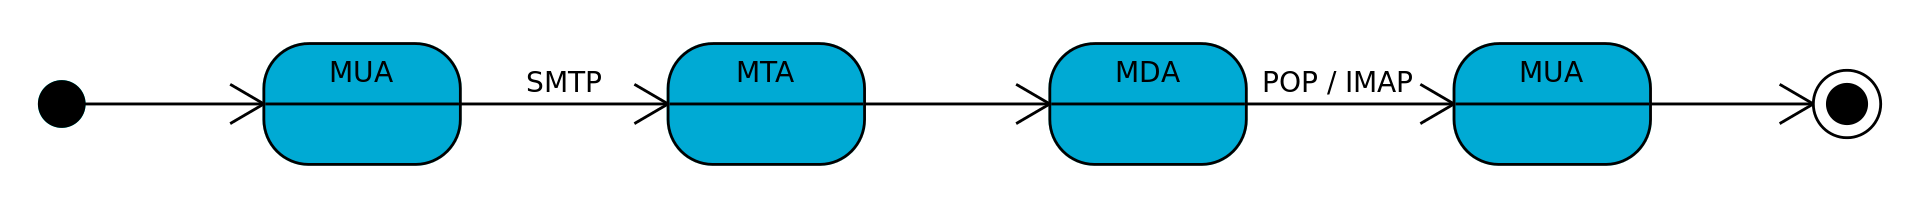
\includegraphics[width=14cm]{images/Etapes_envoi_email.png}
	\centering
	\caption{Le fonctionnement d'un système de mail~\cite{wiki:mailGlobal}}
	\label{fig:mailGlobal}
\end{figure}
\section{Protocoles existants}
Dans cette section je vais analyser les différents protocoles existants afin de sécuriser la messagerie électronique, ainsi que leur implémentation au sein de certains clients mails. De plus je m'intéresserait à la messagerie instantanée afin de voir s'il est possible d'implémenter cela dans un système de mails.
\subsection{PGP}
\paragraph*{Fonctionnement.}
PGP (Pretty Good Privacy ou Assez bon niveau de confidentialité) est un moyen de chiffrer des données (mails, fichiers, …). C’est une méthode de chiffrement hybride (utilise le chiffrement symétrique et asymétrique) qui fonctionne comme montré sur la Figure \ref{fig:PGP_101}. Comme on peut le voir, on tire une clé symétrique aléatoirement qui permettra de chiffrer notre mail avec un chiffrement symétrique comme AES. Ensuite, l'on va chiffrer cette clé symétrique à l'aide d'un chiffrement asymétrique, en utilisant la clé publique du destinataire.

\begin{figure}[h!]
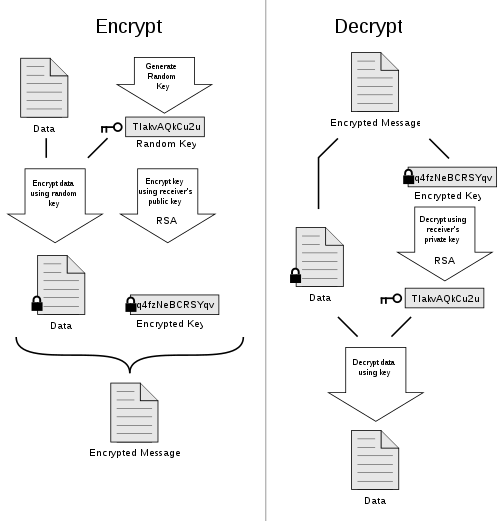
\includegraphics[width=10cm]{images/PGP_101.png}
\centering
\caption{Le fonctionnement global de PGP}
\label{fig:PGP_101}
\end{figure}

Ce fonctionnement hybride est expliqué par la lenteur d’un chiffrement asymétrique sur un certain nombre de données. Ainsi en chiffrant uniquement la clé symétrique qui a servi à chiffrer le message le déchiffrement est bien plus rapide et simple et est effectué typiquement avec un chiffrement symétrique tel qu’AES qui a le droit à des instructions dédiées dans certains processeurs. Contrairement à des chiffrements asymétriques qui sont plus contraignants. Mais il est nécessaire de passer par cette phase asymétrique, on a en effet besoin d'un secret partagé dès le début de la communication si cette méthode n'est pas utilisée.\\
Pour ce qui est des primitives cryptographiques proposées dans la RFC4880~\cite{RFC4880}, elle sont listées ci-après dans la table \ref{table:refPGPAlgos}.
\begin{table}[h!]
	\centering
	\begin{tabular}{||c c c c||}
		\hline
		Symetric & Asymetric & Hash & Compression \\ [0.5ex]
		\hline\hline
		IDEA & RSA & MD5 & ZIP \\
		TripleDES & ElGamal & SHA-1 & ZLIB \\
		CAST5 & DSA & RIPE-MD160 & BZip2 \\
		Blowfish & ECDSA & SHA256 & \\
		AES-128 & Diffie-Hellman & SHA384 & \\
		AES-192 & & SHA512 & \\
		AES-256 & & SHA224 & \\
		Twofish-256 & & & \\
		IDEA & & & \\
		\hline
	\end{tabular}
\caption{Table des algorithmes utilisés par PGP}
\label{table:refPGPAlgos}
\end{table}
Attention MD5 a été anoncé déprecié. Il faut savoir que pour chacune de ces catégories il y a 10 éléments réservés pour des primitives privées/expérimentales.\\
Lorsqu'un mail est chiffré et signé avec PGP, il est d'abord hasher puis ce hash est signé avec la clé privée de l'utilisateur afin de faire une signature digitale. Le message et la signature sera alors chiffrée à l'aide la clé symétrique.\\
L'organisation d'un message PGP se fait via des "paquets" d'informations encodés en base64. La RFC définit bien ces types de paquets, leur fonctionnement et les différents codes associés. Sur le blog de Conrad Irwin\footnote{\url{https://cirw.in/gpg-decoder/}} l'on peut entrer un message et ainsi voir l'organisation d'un message, de clés publiques et de clés privées. Ainsi, je montre un exemple de mail envoyé à plusieurs destinataires dans la figure \ref{fig:PGP_DECODE}. Cela démontre comment fonctionnes PGP, en effet le message étant chiffré avec une clé symétrique, le chiffré sera le même pour tout le monde. Mais afin que tout les destinataires puisses avoir la clé symétrique, la clé est chiffrée à l'aide des clés publiques des différents destinataires (et de la source, pour pouvoir la déchiffrer à l'avenir et ne pas conserver le mail en clair dans la boite d'envoi). À noter qu'avec l'option de \textit{blind copy} (option permettant d'envoyer à un utilisateur un mail sans qu'il sache qu'il a aussi été envoyé é un autre utilisateur), PGP \textit{leak} les receveurs des mails avec leur KeyID qui sera présent dans le message PGP~\cite{BccPrivacy}.\\
\begin{figure}[h!]
	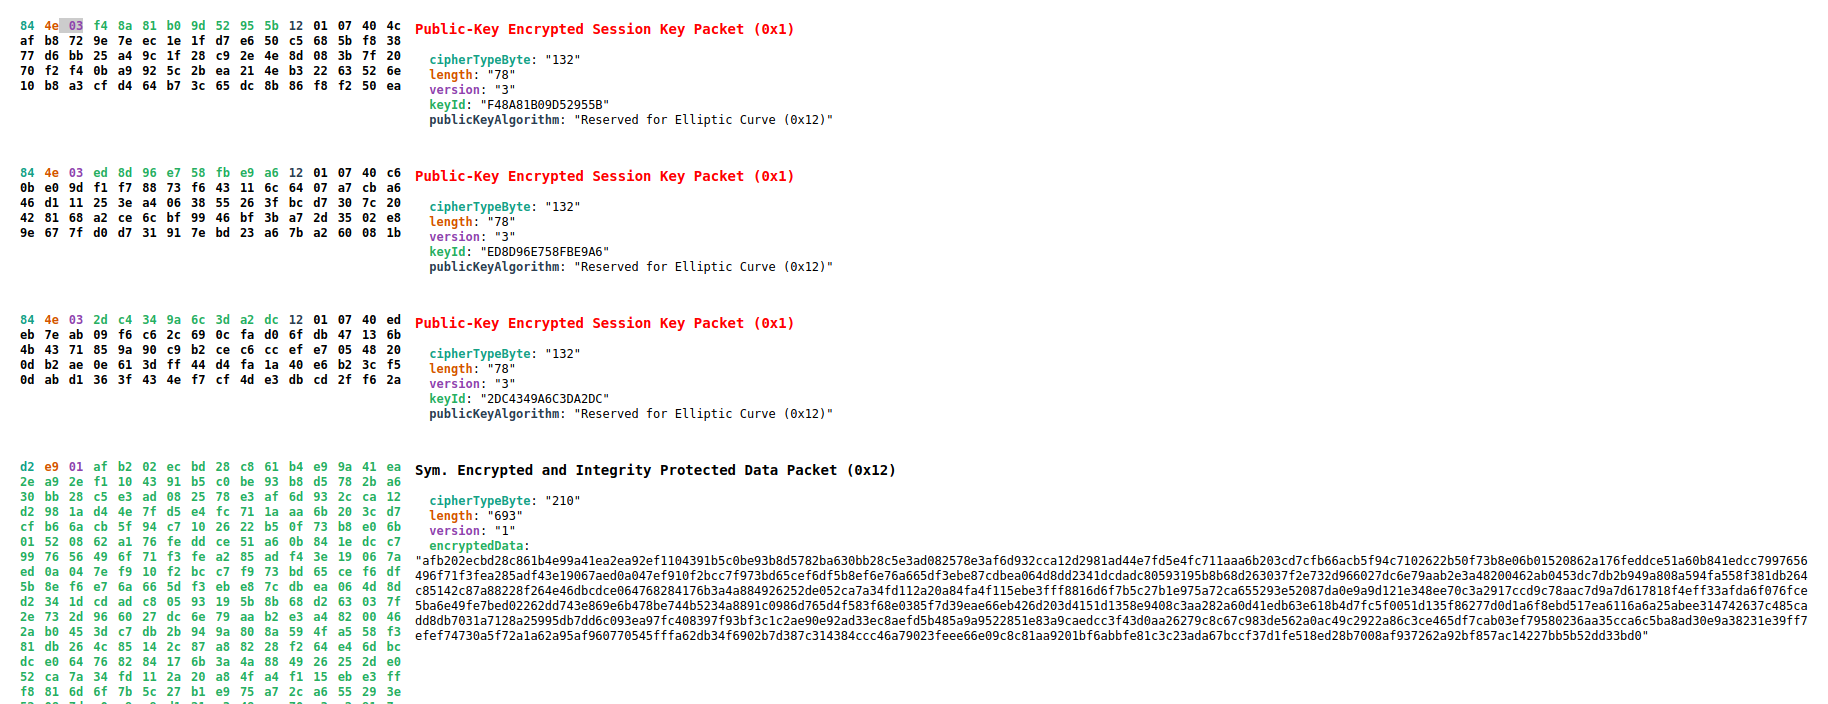
\includegraphics[width=14cm]{images/examplePGPDecode.png}
	\centering
	\caption{Exemple décodage d'un message PGP}
	\label{fig:PGP_DECODE}
\end{figure}
PGP utilise donc un système de clés publiques afin d'envoyer des clés symétriques. Comment obtient-on une clé publique pour envoyer notre message ?\\
Selon certaines utilisations les clés peuvent être obtenues via un serveur de clés, mais cela implique un parti tier auquel il faut faire confiance, ainsi ce qui peut être fait c'est aussi d'avoir son propre serveur de clés. Mais pour être sûr que tel clé appartienne bien à tel utilisateur, PGP a introduit dès ces débuts un système décentralisé de confiance appelé le "Web of Trust". Ainsi, un utilisateur pourra faire confiance à certaine clés d'autres utilisateurs et les signer, puis chacun des utilisateurs aura des clés de confiance et ainsi de suite. Cela permet d'avoir une toile de confiance entres les utilisateurs. Cependant, ce système est difficile à utiliser, il est nécessaire de faire attention à quelles clés les utilisateurs signent et approuvent. Surtout pour les nouveaux utilisateurs qui ne peuvent faire vérifier leurs clés publiques facilement et ne seront donc pas vérifier, c'est pour cela que des "fêtes" de signature de clés sont organisées afin de se rencontrer personnellement et vérifier que tel utilisateur est bien telle personne. Ces évènements sont d'ailleurs possible grâce aux Fingerprint des clés publiques, ce sont des chaines hexadécimales de 20 bytes permettant d'identifier une clé publique plus facilement.\\
SHA-1 est encore beaucoup utilisé pour les certificats d'identité et il a été prouvé que des attaques sur cet algorithme au niveau des collisions peuvent être faites~\cite{DBLP:journals/iacr/LeurentP20} donc à éviter d'utiliser également. Maintenant modifié dans les nouvelles version de GnuPG, ce n'est plus le standrad pour signer les clés publiques d'autres utilisateurs dans le Web Of Trust.\\
Dans la dernière spécification de PGP des moyens de créer des certificate authorities ont été ajouté afin d'avoir un système décentralisé de \textit{trust signatures} à différents niveaux et ainsi pouvoir se baser sur un système qui ressemble à un PKI mais avec une flexibilité sur les CAs (utilisateurs) auxquels on fait confiance ou non.
\paragraph*{Propriétés cryptographiques.}
PGP a surtout été crée pour fournir du \textbf{chiffrement de bout-en-bout} afin de résoudre les problèmes de transmissions en clairs entre les MTAs et le stockage des mails en clair dans les MDAs. Ainsi même lors d'une récupération de mails sur un serveur les mails seraient chiffrés. Ensuite PGP propose de signer ou non ses mails ce qui amène donc de la \textbf{répudiation} (si non-signé, le mail ne pourra pas être utilisé pour prouver qu'il a été envoyé par telle personne) et \textbf{non-répudiation} (mail signé, ainsi l'on peut prouvé que l'envoyeur a bien envoyé le mail).\\ 
Le problème qui est souvent reproché à PGP c'est qu'il n'implémentes pas de \textbf{Forward Secrecy}. La \textit{Forward Secrecy} permet d'affirmer que si l'on a une brèche à un instant $t$, et qu'un attaquant récupère notre clé privée, il ne pourra pas déchiffrer les anciens messages chiffrés avant l'instant $t$.
\paragraph*{Utilisation.}
Lors des tests l’utilisation la plus simple possible a été utilisée pour voir si un utilisateur lambda pouvait arriver à mettre en place ce genre de sécurité. Il s’est avéré que cela était assez simple au départ, mais dès lors que l'on veut envoyer un mail chiffré à un correspondant cela se complique. Uniquement l'installation d'un Add-On sur le logiciel de messagerie (Thunderbird dans ce cas) s’appelant Enigmail a été nécessaire. Ensuite Enigmail a généré les clés PGP (de manière totalement automatisée). Puis l'envoi d'un mail se fait simplement et rapidement via des icônes et des options dans le client mail. Cependant c’est très opaque et on ne sait pas ce qu'Enigmail fait réellement derrière les décors. L’utilisateur doit encore choisir s’il veut chiffrer ses mails ou non. De plus, Enigmail utilise Autocrypt, un système permettant d'envoyer la clé publique directement dans le mail. Pour les clés, Enigmail les envoie sur des serveurs de clés par défaut. Il va aussi interrogé ces serveurs si une clé publique pour un destinataire est disponible dessus lors du chiffrement d'un message. Ces serveurs sont les suivants : keys.opengpg.org (vks), hkps.pool.sks-keyservers.net (hkps), pgp.mit.edu (hkps). vks (Verifying Keyservers) et hkps (HTTP keyserver protocol over TLS) sont des interfaces avec des serveurs de clés afin d'enregistrer des nouvelles clés ou trouver une clé sur le serveur par différents moyens (email, key-id, fingerprint). Les clés générées ont été générées avec les algorithmes de courbe elliptique EdDsa 4096bits par défaut, et dans les paramètres avancés il est possible de choisir entre cet algorithme et RSA.
\subsection{S/MIME}
\label{protocols:SMIME}
\paragraph*{Fonctionnement.}
S/MIME (Secure/Multipurpose Internet Mail Extensions) se base sur un système de PKI (Public Key Infrastructure) pour chiffrer et signer les mails.Dans une telle infrastructure les CAs (Certificate Authorities) garantissent que les certificats décrivent bien l'entité.\\
MIME est un standard qui étend le format de mail standard afin de pouvoir transmettre des données plus complexes que le format ASCII. En effet, cela permet de transmettre d'autres sets de caractères et la possibilité de transmettre des fichiers joints audio, vidéo, images, programmes aux emails. MIME permet de séparer le message en partie, c'est d'ailleurs là dessus que l'attaque EFAIL (c.f. section \ref{attacks:EFAIL}) s'appuie. Ces parties ont différent format de données et le message MIME est défini selon un type parmi : mixed, digest, alternative, related, report, signed, encrypted, form-data, mixed-replace, byteranges. Ces types de contenu sont là pour définir de quoi est composé le message et comment le décoder, fonctionnant via une notion de frontières entres les différentes parties.\\
Dans ce contexte S/MIME vient ajouter un type MIME \textit{application/pkcs7-mime}, un format de donnée qui enveloppe une entité MIME afin de la chiffrer, puis cette enveloppe chiffrée est ensuite le contenu de ce nouveau type. Cette enveloppe  Pour les signatures S/MIME utilisera plus le signatures détachées et le type \textit{multipart/signed} pour cela ou encore \textit{application/x-pkcs7-signature}. Anciennement c'était effectivement le format de message PKCS\#7 utilisé pour le format des messages chiffrés. Cependant, à l'heure actuelle c'est la spécification de CMS (Cryptographic Message Syntax) qui est utilisé dans ces types MIME.\\
Afin de commencer à signer des messages avec S/MIME et pouvoir recevoir des messages chiffrés il faut un certificat. Ce certificat peut être obtenu soit par une autorité de certification interne ou une autorité externe. Ces certificats peuvent être de classe 1 (vérification que le propriétaire du certificat peut recevoir des messages envoyés au "From:" de ses messages) ou de classe 2 avec plus de précisions sur le propriétaire du certificat.\\
Pour signer un message, S/MIME va utiliser la clé privée lié au certificat de la source, ainsi le message va être signé avec la primitive adéquate par rapport aux informations du certificat. Puis la signature sera envoyée avec le certificat, afin que le destinataire puisses vérifier la signature à l'aide du certificat. Et vérifier le certificat avec un CA.\\
Comme le présente la RFC8551~\cite{RFC8551}, le chiffrement effectué par S/MIME s'approche de celui fait par PGP, en effet S/MIME va chiffrer la clé de chiffrement symétrique (Content Encryption Key dans CMS) une fois par destinataire en utilisant la clé publique authentifiée par leur certificat respectif et aussi une fois pour la source du message (afin de pouvoir relire le message envoyé à l'avenir). Les algorithmes qui doivent être pris en charge dans CMS sont les suivants selon la RFC8551 dans la table \ref{table:refSMIMEAlgos}.\\
\begin{table}[h!]
	\centering
	\caption{Table des algorithmes utilisés par S/MIME}
	\label{table:refSMIMEAlgos}
	\begin{adjustbox}{width=\textwidth}
		\begin{tabular}{||c c c c||}
			\hline
			Symetric & Asymetric & Hash & Signature \\ [0.5ex]
			\hline\hline
			AES-128 CBC & ECDH sur P-256 & SHA-256 & ECDSA (courbe P-256 et SHA-256) \\
			ChaCha20-Poly1305 & ECDH  avec HKDF-256 & SHA-512 & EdDSA (courbe 25519 avec PureEdDSA mode) \\
			AES128-GCM & RSA & & RSA PKCS \#1 v1.5 avec SHA-256 \\
			AES256-GCM & RSAES-OAEP & & RSASSA-PSS avec SHA-256\\
			\hline
		\end{tabular}
	\end{adjustbox}
	
\end{table}
\paragraph*{Propriétés cryptographiques.}
S/MIME est aussi crée pour établir un \textbf{chiffrement bout-en-bout} et ainsi éviter de révéler trop d'informations lors d'une brèche tel que dans un MDA. 
\textbf{Authentification} et \textbf{intégrité} du message en utilisant la signature digitale, en plus de \textbf{non-répudiation} grâce à celle-ci. Le fait d'avoir le message chiffré de bout en bout permet un certain respect de la vie privée, on ne peut voir les données envoyées.
\paragraph*{Utilisation.}
Pour utiliser S/MIME et avoir des exemples et références de certificats j'ai essayé 2 fournisseurs \textbf{gratuits} pour les certificats S/MIME.
J'ai testé un plugin firefox qui permet d'avoir des certificats pour GMail et envoyer des mails signés et chiffrés à l'aide de S/MIME. La clé privée est générée par l'extension localement et n'est pas sauvegardée dans un cloud, il est possible de la sécurisé à l'aide dune passphrase. Cependant les certificats ne sont pas vérifier correctement comme on peut le voir à la réception dans MeSince (le prochain programme testé) à la figure \ref{fig:SMIME_MeSinceProblem}. Le certificat utilise RSA avec SHA256 pour la signature des messages.
\begin{figure}[h!]
	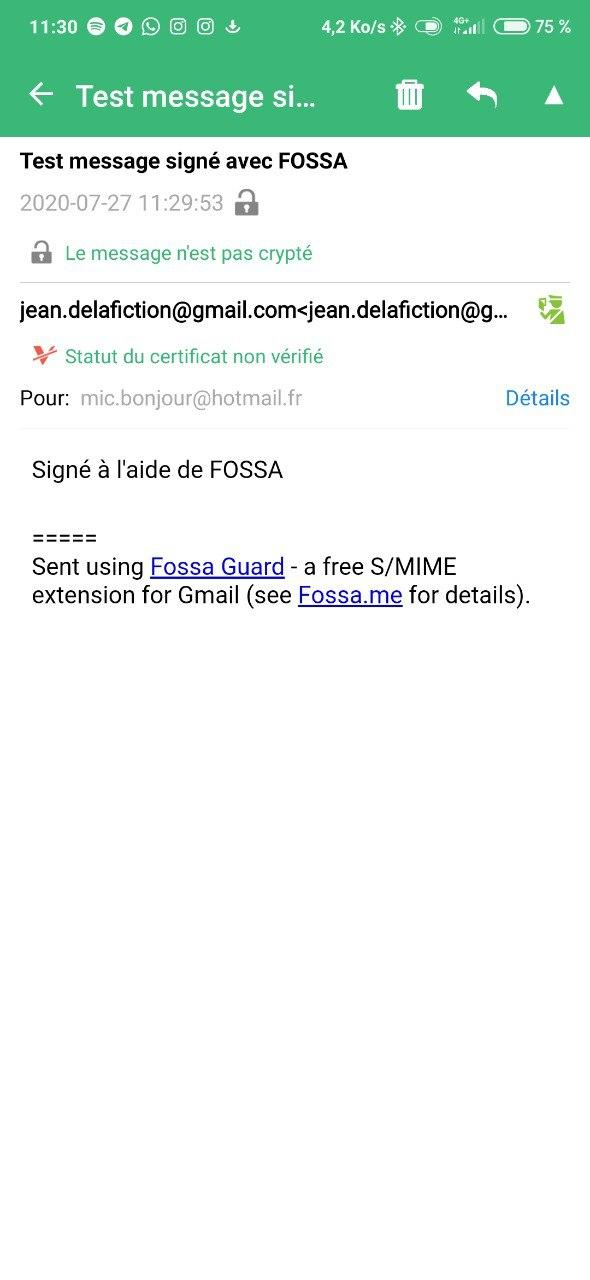
\includegraphics[width=10cm]{images/SMIME_FossaProblem.jpg}
	\centering
	\caption{Erreur de vérification pour Fossa}
	\label{fig:SMIME_FossaProblem}
\end{figure}
Pour tester S/MIME, j'ai aussi lié un compte \url{https://www.mesince.com}. En effet, ce service permet d'utiliser S/MIME afin de chiffrer et signer ses mails, et ils fournissent les certificats, seulement il ne fonctionnait pas avec Gmail. De plus le service fourni n'a pas fonctionné pour se loguer et récupérer son certificat, ainsi le certificat a été généré et peut être utilisé par leur application mobile pour envoyer des mails signés et chiffrés mais je ne peux pas le voir. Sur l'application mobile il n'y a pas moyen de vérifier la clé générée.
Attention cependant le même problème qu'avec Fossa arrive comme je le montre dans la figure \ref{fig:SMIME_MeSinceProblem}, par contre l'avertissement n'est pas très voyant au sein de Gmail. Les certificats utilisent RSA avec SHA256 pour la signature des messages.
\begin{figure}[h!]
	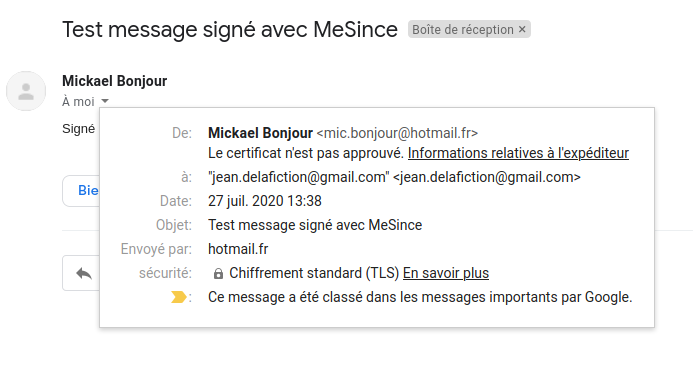
\includegraphics[width=15cm]{images/mesince_problem.png}
	\centering
	\caption{Erreur de vérification pour MeSince}
	\label{fig:SMIME_MeSinceProblem}
\end{figure}
MeSince informe que la clé privée est automatiquement sauvegardée dans leur cloud sécurisé, ce qui n'est pas forcément une bonne nouvelle, de plus la clé est générée automatiquement donc aucune vérification de la part de l'utilisateur.
Cependant ces 2 tests effectués ne représentent pas vraiment une utilisation réelle de S/MIME, en effet, le meilleur moyen de tester S/MIME aurait été d'avoir un nom de domain à soi et de générer des certificats S/MIME pour une adresse privée. Ensuite d'importer ses certificats et ses clés dans le client mail utilisés.
% TODO revoir PEP ?
\section{Implémentations existantes}
Dans cette section je présentes certaines implémentations des protocoles discutés dans la section précédente, plus particulièrement PGP.
\subsection{Protonmail}
\paragraph*{Revendications.}
Protonmail revendique beaucoup de propriétés cryptographiques, tel que le zero-access encryption (lors de la réception d'un message externe chiffré ou non Protonmail le chiffrera avec la clé publique de l'utilisateur pour ne plus y avoir accès dans le futur). Et l’end-to-end chiffrement + zero-knowledge pour les messages sécurisés, même avec leur fonctionnalité de chiffrement vers l'extérieur utilisant AES256-GCM. Possibilité de mettre une date d'expiration sur un mail afin que le destinataire ne puisses le lire que dans un temps imparti.
Pour l'authentification Protonmail utilise une manière fortement sécurisée (SRP) pour ne pas avoir d'informations direct sur le mot de passe de l'utilisateur.
Protonmail chiffre automatiquement les mails d'un utilisateur Protonmail à un autre via PGP.
\paragraph*{Fonctionnement.}
Protonmail a plusieurs modes de fonctionnement dépendant du destinataire final. En effet de Protonmail à Protonmail les mails sont chiffrés à l'aide de PGP automatiquement. L'on peut utiliser Protonmail pour utiliser PGP si l'on a la clé de notre destinataire par exemple. Et l'on peut écrire un mail chiffré à quelqu'un qui n'utilise pas PGP grâce à une fonctionnalité de chiffrement vers l'extérieur.
Cette fonctionnalité enverra une URL au destinataire qui, en la consultant, pourra déchiffrer le mail en utilisant un mot de passe communiqué auparavant de manière sécurisées entres les deux partis. Un exemple de mail utilisant cette fonctionnalité est présenté dans la figure \ref{fig:ProtonmailPres}.
\begin{figure}[h!]
	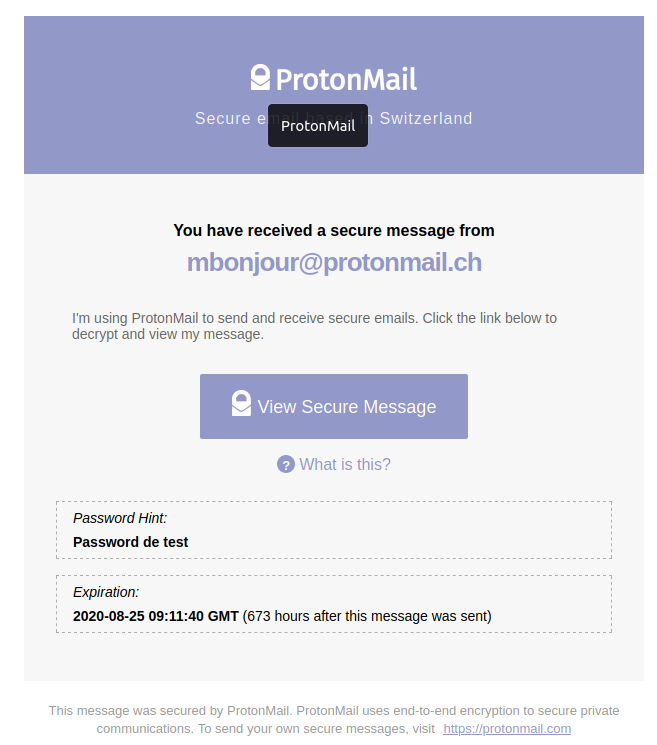
\includegraphics[width=10cm]{images/protonmailPresentation.png}
	\centering
	\caption{Présentation d'un email chiffré Protonmail}
	\label{fig:ProtonmailPres}
\end{figure}
\paragraph*{Open Source.}
Leur code est open-source afin d'avoir une validation externe, de plus ils ont un programme de Bug Bounty pour les chercheurs. Ils ont largement contribué au projet d'intégration openpgp en javascript et en Go.

\paragraph*{Utilisation.}
Lors de l'utilisation de protonmail, l'analyse des clés PGP générées à montrer qu'elles utilisent RSA. Pour envoyer ou recevoir des messages via PGP, Protonmail le fait de manière très transparente. Apparemment utilisant les mêmes serveurs de clés cités plus haut pour Enigmail, en effet, les 2 emails de tests ont pu s'envoyer des messages sans s'envoyer les clés au préalable.\\
Sensation de sécurité en utilisant Protonmail, en effet un mot de passe est utilisé pour chiffrer notre boite mail, pratique si une brèche survenait au niveau du stockage protonmail. De plus, la technologie utilisée pour l'authentification et les mots de passe et SRP. Permettant de ne pas avoir de hashs de mots de passe stockés chez Protonmail.\\
Par contre la génération de la clé privée à la création du compte est assez obscure mais de l'information est disponible sur le site de protonmail\footnote{\url{https://protonmail.com/support/knowledge-base/how-is-the-private-key-stored/}}.\\
\paragraph*{Critiques.}
Protonmail est très critiqué de manière générale sur les réseaux sociaux. De plus une réponse au chercheur Nadim Kobeissi~\cite{DBLP:journals/iacr/Kobeissi18a} avait été formulée par Protonmail suite à son papier sur l'insécurité le leur webmail. Cependant, ils sont surtout critiqué sur les réseaux sociaux par des chercheurs en sécurité\footnote{\url{https://twitter.com/FiloSottile/status/1277068367728435202}} pour leur publicité mensongère, en effet, leur page d'accueil indiquait une sécurité pour \textbf{tous} les email sortants. Ce qui n'est pas le cas, uniquement les mails intentionnellement chiffré à l'aide de PGP ou chiffré vers l'extérieur sont chiffré. L'annonce ne représentait donc pas la réalité, ce qui peut être mal interprété par les utilisateurs. Après vérification la page d'accueil a bien été modifiée pour ne plus inclure la mention de chiffrement automatique pour tout les emails. Le commentaire fait référence aussi à d'autres points :
\begin{itemize}
	\item Ingère les emails en plaintext - par rapport à leu politique de zero-access, ils ont au moins une fois accès au plaintext d'un email non chiffré.
	\item Pas de réels solutions pour du chiffrement vers l'extérieur - La solution amenant l'utilisateur distant à se connecter à leur service pour déchiffrer un message n'est pas une solution viable.
	\item Utilise de la cryptographie dans le navigateur non validée - Modules cryptographiques servis par les serveurs de Protonmail, on revient ici aux revendications de ce papier~\cite{DBLP:journals/iacr/Kobeissi18a}. Malgré cela une solution existe désormais, utiliser un bridge disponible à \url{https://github.com/ProtonMail/proton-bridge}.
	\item Agit comme un serveur de clés, sans transparence de clés - Suite à la mise en place d'un serveur de clés pour chercher les clés PGP d'utilisateur Protonmail pas de transparence sur ce serveur n'a été communiqué.
\end{itemize}
\subsection{Tutanota}
\paragraph*{Fonctionnement.}
Tutanota est un client mail sécurisé, il permet de chiffrer les mails vers l'extérieur. Cela en utilisant AES128-CBC selon ce que le code github analysé.
\paragraph*{Utilisation.}
L'utilisation de Tutanota est facile, en effet Tutanota utilise le même principe que Protonmail pour le chiffrement vers l'extérieur. En chiffrant le mail et en le gardant sur ses serveurs puis en envoyant un mail au destinataire comme celui présenté dans la figure \ref{fig:TutanotaPres}.
\begin{figure}[h!]
	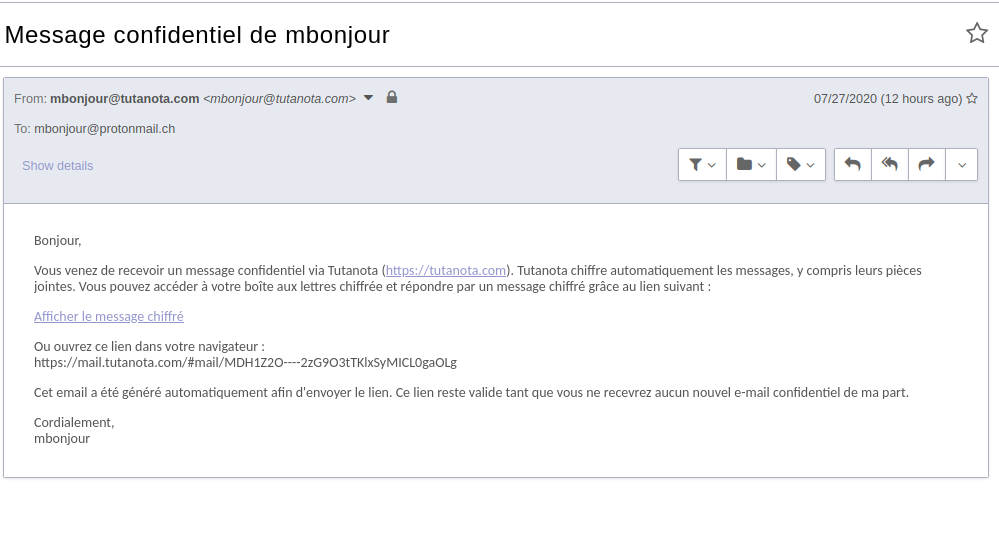
\includegraphics[width=14cm]{images/tutanotaPresentation.png}
	\centering
	\caption{Présentation d'un email chiffré Tutanota}
	\label{fig:TutanotaPres}
\end{figure}
% TODO : Revoir
%\subsection{Bitmessage}
\section{Attaques existantes}
Présentation des attaques faites sur les différents systèmes présentés jusqu'ici ainsi que leur fonctionnement global.
\subsection{Défauts webmails}
Selon un chercheur~\cite{DBLP:journals/iacr/Kobeissi18a} l'infrastructure de Protonmail aurait des failles via son webmail. Mais son papier est en fait plus général et parle des webmails en règle générale.
Il part du principe que les serveurs de Protonmail ne sont pas des serveurs à faire confiance, pour ainsi prouver le zero-knowledge de Protonmail. Par contre, le fait qu'il ne peuvent pas être mis en confiance est un problème selon lui, car c'est ces serveurs qui vont délivrer le code d'OpenPGP afin de faire le chiffrement. 
Cela indique que si Protonmail était corrompu le fait d'avoir le code délivré par Protonmail pourrait avoir des effets néfastes. Comme p.ex l'extraction de la clé privée PGP. La conclusion est que dès le moment où vous avez utilisé une fois le webmail de protonmail la clé PGP pourrait être corrompue ou connue de Protonmail.
\subsection{EFAIL}
\label{attacks:EFAIL}
Malgré ces sécurités qui pourraient être mises en place à l’heure actuelle, une attaque nommée EFAIL~\cite{DBLP:conf/uss/PoddebniakD0ISF18} a été faite en 2018. En effet cette attaque a seulement été mitigée en évitant d’afficher les contenus HTML et les images dans les boites mails de base. Car le problème vient de là principalement, des problèmes sont liés aussi aux modes de chiffrement utilisé (typiquement CBC et CFB pour S/MIME et PGP respectivement) grâce à des "gadgets".
Cette attaque permet en fait d'injecter une image dans l'HTML du message, puis faire en sorte de récupérer le contenu du message déchiffrer dans l'URL. Ceci est possible grâce au multi parties de MIME et en les abusant afin d'entourer le message chiffré d'une balise \textit{img} et de mettre en source le message qui sera déchiffré selon les règles de MIME. Ainsi l'attaquant aura le message déchiffré dans l'url qu'il peut contrôler. Cette attaque exploite en fait une erreur par rapport à la gestion des messages utilisants HTML et multipart/mixed, il faudrait en effet vérifier dans ces cas que le document HTML est un document entier. Ainsi que de ne pas traiter le contenu chiffré de la même origine que du contenu non protégé. La spécification~\cite{RFC8551} S/MIME a aussi mise à jour pour implémenter des chiffrements authentifiés et remplacer CBC qui permettait des attaques par gadgets.
\subsection{SHA-1 Shambles}
Récemment~\cite{DBLP:journals/iacr/LeurentP20} une attaque sur SHA-1 avec un préfixe choisi. Cette attaque permet de se faire passer pour quelqu'un d'autre grâce à une attaque par préfixe choisi sur SHA-1. SHA-1 était en effet l'algorithme de hachage par défaut pour signer les clés d'autres utilisateurs dans le \textit{Web Of Trust}.
\section{Signal}
L'analyse s'est faite aussi pour la messagerie instantanée à cause de sa ressemblance avec la messagerie électronique. 
\subsection{Fonctionnement}
Le fonctionnement de Signal est complexe à expliquer, ainsi la figure \ref{fig:signal} sera plus parlante pour expliquer le Diffie-Hellman Ratchet. Ce premier Ratchet permet d'utiliser Diffie-Hellman afin d'avoir une première sortie synchronisée entre l'envoi et la réception d'un utilisateur. Au début de la discussion Bob va envoyer sa clé publique et Alice va pouvoir commencer son premier Ratchet en générant elle aussi une paire de clés Diffie-Hellman. On verra dans la figure suivante ce qu'il se passe ensuite pour le chiffrement des messages mais une fois cett opération finie, Alice envoi sa clé publique précedemment générée à Bob pour qu'il puisses générer la même clé partagée à l'aide de Diffie-Hellman et ainsi déchiffrer le contenu en s'aidant du Deuxième Ratchet.
\begin{figure}[h!]
	\centering
	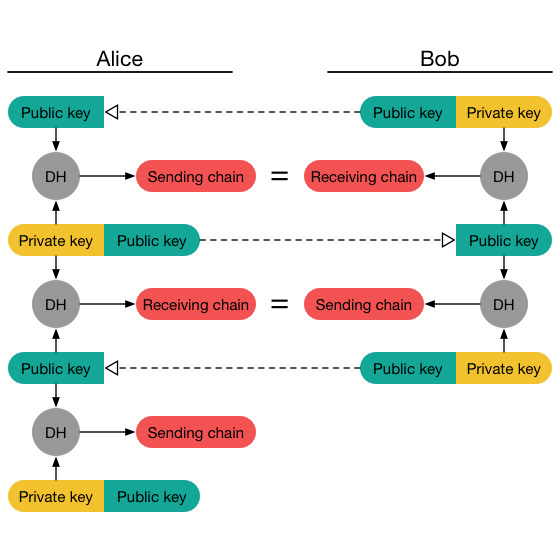
\includegraphics[width=8cm]{images/signalFonctionnement.png}
	\caption{Schéma fonctionnement du DH Ratchet\cite{doubleratchet}}
	\label{fig:signal}
\end{figure}
Par contre l'image est une simplification, la clé DH ne va pas être utilisée tel quel, elle sera insérée dans une KDF avec une Root Key (partagée à l'aide de X3DH) qui sortira la prochaine Root Key et la Receiving/Sending Chain Key qui sera donnée au deuxième Ratchet.\\
Le deuxième ratchet va générer une clé pour chaque message/batch de messages afin d'envoyer un message chiffré avec le moins d'utilisation de la même clé possible. Ainsi la forward secrecy est plus forte.Dans cet exemple on voit qu'Alice a envoyé un message chiffré à l'aide d'A1 puis qu'elle a reçu un nouveau DH Ratchet de Bob qui lui a permis de générer sa prochaine Receiving Chain Key et de déchiffrer les messages que Bob a envoyé (B1).
\begin{figure}[h!]
	\centering
	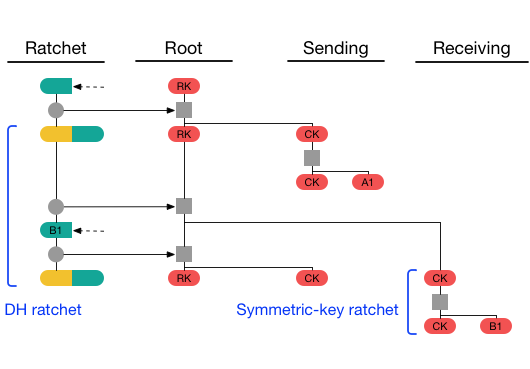
\includegraphics[width=10cm]{images/secondRatchet.png}
	\caption{Schéma fonctionnement du deuxième Ratchet\cite{doubleratchet}}
	\label{fig:signalSecond}
\end{figure}
\subsection{Propriétés cryptographiques}
Signal a de nombreux avantages concernant les propriétés cryptographiques qu'il promet. En effet le \textit{Double Ratchet} permet de la \textbf{Break-in recovery}, a une \textbf{Perfect Forward Secrecy}, \textbf{End-to-End encryption}, \textbf{Non-Répudiation}.
\subsection{Problèmes d'intégrations}
Le problème avec le protocole Signal quant à mes besoins niveaux mails est la \textit{perfect forward secrecy} qui est très forte. En effet comme vu dans le chapitre précédent il utilise une clé par message grâce au \textit{Double Ratchet}. Cependant ce fonctionnement comporte un gros problème en rapport aux mails, en effet si l'on veut pouvoir récupérer les anciens mails reçus/envoyés cela devient vraiment compliqué. La \textit{forward secrecy} est une propriété utile dans un système de mail, mais il faut pouvoir aussi récupérer les messages facilement si l'on connait la clé privée. Alors qu'avec ce système de Double Ratchet il nous faudrait enregistrer chaque Diffie-Hellman ratchet pour reconstruire toute les clés utilisée.
\section{Compromis}
Pour passer à l'implémentation concrète d'un nouveau protocole il faut faire des compromis et aller chercher dans des primitives moins connues.\\
Je suis tout de même rester sur un système de clés publiques comme PGP le fait. Cependant cette primitive a une identité propre à chaque clé publique ce qui évite un systéme de certificat trop complexe comme S/MIME.\\
De plus pour avoir une \textit{forward secrecy} l'on peut ajouter une notion de temps ou de token à l'ID pour chaque batch de messages.
\subsection{Résultats des recherches}
Comme mentionné avant les recherches ont beaucoup été orientées sur le protocole Signal qui a une très bonne forward secrecy, résilience et break-in recovery. Cependant le problème avec l'utilisation des mails c'est d'avoir envie de consulter tout ces mails depuis n'importe quel appareil. Ce n'est malheureusement pas le cas avec Signal à moins de conserver une \textit{root key} quelque part qui ferait s'effondrer les caractéristiques principales du protocole.\\
S/MIME est la solution prédominante pour s'envoyer des mails chiffrés cependant il est compliqué de l'utiliser. Il et en effet difficile d'obtenir un certificat pour envoyer des mails et échanger avec une autre personne ayant S/MIME. De plus la complexité d'un système de PKI et l'overhead induit est assez conséquent.\\
En faisant quelques essais PGP de mon côté je me suis heurté à beaucoup de difficultés et de problèmes avec les clés PGP, notamment pour se les échanger mais pour envoyer ensuite ce n'est pas si complexe, le problème étant de bien voir les primitives utilisées pour chiffrer/signer notre email, en effet les solutions \textit{plug-and-play like} ne permettent pas une gestion précise des primitives cryptographiques utilisées, ce qui pourrait induire à des primitives par défaut non sécurisées, comme l'a démontré EFAIL(c.f. \ref{attacks:EFAIL}).
\section{Primitives}
Présentation des primitives considérées pour implémenter un système de messagerie sécurisée. Cette section présente un aperçu des primitives analysées, pourquoi je l'ai ou non retenue et leur fonctionnement en quelques mots.
\subsection{Primitives analysées}
Les primitives analysées sont présentées si après. Elles ont en commun de s'appuyer sur un principe basé sur l'identité. C'est très pratique dans un système de mail car une identité peut-être très vite définie par le biais d'une adresse email. Voici donc les technologies auxquelles les recherches se sont portées :
%TODO : Expliquer les différentes primitives
\begin{itemize}
	\item Identity based encryption~\cite{DBLP:conf/crypto/Shamir84}, primitive instaurant en premier le binding entre un ID et le chiffrement, ceci afin d'éviter les infrastructures complexes de PKI. Cependant, cette primitive introduit le \textit{key escrow problem}, un problème inhérent de la construction qui nécessite un KGC générant les clés privées pour les utilisateurs et qui en apar la conséquente connaissance.
	% TODO remettre ce qu'Alex avait envoyé A Forward-Secure Public-Key Encryption Scheme∗
	%\item HIBE - Hierarchical Identity Based encryption~\cite{DBLP:conf/eurocrypt/HorwitzL02}
	\item Certificateless PKC~\cite{DBLP:conf/asiacrypt/Al-RiyamiP03}
\end{itemize}
\subsection{Primitive choisie}
- Certificateless PKC~\cite{DBLP:conf/asiacrypt/Al-RiyamiP03}\\
 Cette primitive a été choisie car elle est similaire à de l'identity based encryption avec un ID pour désigner une clé publique. Le problème avec l'identity based encryption c'est le fait que le serveur central génère la clé publique et la clé secrète de l'utilisateur, cela amène ce qu'on appelle le \textit{key escrow} problème. C'est le fait qu'une entité connaisse à elle seule toutes les clés de tout les utilisateurs. Ce problème est résolu dans le certificateless en introduisant des \textit{Partial Private Keys} permettant d'avoir une clé secrète partiellement générée par le serveur (KGC - Key Generation Center) et par l'utilisateur puis assemblée pour former la clé privée seulement connue de l'utilisateur. De plus, cette primitive a l'avantage de ne pas introduire de certificats et ainsi évites la complexité d'une infrastructure de PKI (Public Key Infrastructure).
\section{Recherches sur la primitive}
\label{sec:primitiveSearch}
Dans cette section je vais introduire les détails techniques et les principes mathématiques utilisés. De plus, le choix de schéma parmi tous ceux analysés est détaillé ici. Ainsi que des précisions sur certains principes introduit par ce schéma.
\subsection{Principes mathématiques}
Les variantes de \textit{Certificateless Cryptography} choisies utilisent un concept appelé les \textit{pairings} ou \textit{bilinear map groups}. Les informations suivantes ainsi que le choix de la librairie découle surtout du livre \textit{Guide to Pairing-Based Cryptography}~\cite{bookPairing}.
Des groupes tels que $\mathbb{G}_1, \mathbb{G}_2, \mathbb{G}_T$ d'un ordre premier \textit{p} pour lesquels il existe un mapping $e : \mathbb{G}_1 \times \mathbb{G}_2 \rightarrow \mathbb{G}_T$ avec les propriétés suivantes :\\
1. Bilinéarité : $e(g^a, h^b) = e(g, h)^{ab}$ pour tout $(g,h) \in \mathbb{G}_1 \times \mathbb{G}_2$ et $a,b \in \mathbb{Z}$;\\
2. Non-dégénérescence : $e(g,h) \neq 1_{\mathbb{G}_T} $ tant que $g,h \neq 1_{\mathbb{G}_{1,2}}$;\\
Plusieurs types de Pairings existent :\\
\begin{itemize}
	\item \textbf{Type 1} : Lorsque $\mathbb{G}_1 = \mathbb{G}_2$;
	\item \textbf{Type 2} : Lorsque $\mathbb{G}_1 \ne \mathbb{G}_2$ mais qu'un isomorphisme $\phi : \mathbb{G}_1 \rightarrow \mathbb{G}_2$ est connu, mais pas dans l'autre direction.
	\item \textbf{Type 3} : Lorsque $\mathbb{G}_1 \ne \mathbb{G}_2$ et qu'aucun isomorphise est connu entre $\mathbb{G}_1$ et $\mathbb{G}_2$, dans n'importe quelle direction.
\end{itemize}
Les différents schémas analysés utilisent souvent les pairings de Type 1, cependant la courbe utilisée, et RELIC me permet de faire des Type 3. Une conversion est faite dans les schémas choisis comme vu ci-après. En effet, les type 3 sont des pairings plus efficients avec des courbes plus petites tandis que les type 1 étaient plus utilisé dans les débuts de la \textit{Pairing Based Cryptography}.
\subsection{À savoir}
\label{subsec:asavoir}
Avant d'analyser les différents schémas, il faut connaître certaines notions présentes dans les tableaux comparatifs afin de mieux les comprendre. Liste non exhaustive de ces notions et de leurs significations et faites ici.
\paragraph*{Types.}Les types présentés peuvent être soit \textbf{concret} soit \textbf{générique}. Les types concrets sont des schémas qui présentent leurs algorithmes en utilisant des calculs bien établis et présentent l'entierté du fonctionnement de leur schéma, tandis que les schémas présenté génériques peuvent s'appuyer sur d'autres problèmes et se baser sur des algorithmes déjà existants.\\
\paragraph*{Modèle de sécurité.} Ces modèles définissent sur quoi le schéma va se reposer pour établir sa sécurité et comment il va l'évaluer face à un adversaire. À nouveau il existe deux modèles présents dans les schémas analysés, le \textit{Random Oracle Model} et le \textit{Standard Model}. Le \textit{Random Oracle Model} se base sur des oracles aléatoires mais est un peu controversé, en effet l'aléatoire cryptographiquement sûr est difficile à atteindre, ainsi habituellement le \textit{Random Oracle Model} implémente ces oracles via des fonctions de hachage. Le modèle standard se base lui sur des problèmes mathématiquement difficiles tel que DDH (Decisional Diffie Hellman). \\
\paragraph*{Modèle d'adversaires.}
Pour évaluer les schémas de certificateless public key cryptography il y a différents niveaux de sécurité établis pour 2 types d'adversaires différents. Ces adversaires ont été décrits dans le papier d'Al-Riyami-Paterson~\cite{DBLP:conf/asiacrypt/Al-RiyamiP03} pour la première fois afin de prouver que leur schéma était IND-CCA sûr dans le modèle Standard. Ces deux adversaires ont été définit comme suit :
\begin{itemize}
	\item Type I (\textit{outsider adversaries}) est permis de remplacer des clés publiques, obtenir des clés partiels privées, et des clés privées puis faire des requêtes de déchiffrements.
	\item Type II (\textit{honest but curious KGC}). L'adversaire de Type II est en fait un KGC connaissant la Master Secret Key et qui peut donc générer des PPK, obtenir des clés privées et faire des requêtes de déchiffrement tout en faisant confiance à ce KGC pour pas qu'il ne remplace de clés publiques.
\end{itemize}
Pour chacun des types d'adversaires il existe différents niveaux de sécurité comme définit dans le livre \textit{Introduction to Ceritifcateless Cryptography}~\cite{bookIntroCertificateless}. Ces différents niveaux sont modélisés comme suit : \\

%TODO : Remplir avec infos du livre sur les différents niveaux
\subsection{Schémas Certificateless de Chiffrement}
Pour choisir parmi les nombreux schémas existants en certificateless pour le chiffrement j'ai établi un tableau comparatif des différentes manières de faire, inspiré de~\cite{bookIntroCertificateless}. En suivant ce tableau je me suis rendu compte que la construction de Dent-Libert-Paterson~\cite{DBLP:conf/pkc/DentLP08} était probablement la plus adaptée en vue des propriétés qu'elle présentait. Le tableau se trouve en annexe \ref{ch:fichiers}.

\subsection{Détails techniques}
Les détails techniques sur le chiffrement avec la \textit{Certificateless Cryptography}.
Le chiffrement se base sur le problème difficile \textit{The Decision 3-Party Diffie-Hellman Problem} (3-DDH). \\C'est de décider si $T =g^{abc} ayant (g^a, g^b, g^c, T) \in \mathbb{G}_4$.\\
Pour expliquer les détails techniques je vais ici montrer les calculs faits dans le schéma choisi~\cite{DBLP:conf/pkc/DentLP08} et les expliquer, cependant dans le schéma il est noté les calculs avec $\mathbb{G} \times \mathbb{G} \rightarrow \mathbb{G}_T$ mais il est mentionné que c'est facilement adaptable pour $\mathbb{G}_1 \times \mathbb{G}_2 \rightarrow \mathbb{G}_T$ ce que j'ai fait. De plus, la conversion vers un groupe additif (travaillant sur les courbes elliptiques) est faite afin que les calculs ici puissent être lus avec mon implémentation :\\
\textbf{Setup($1^k, n$) :} Avec $\mathbb{G}_1, \mathbb{G}_2, \mathbb{G}_T$ avec un ordre $p > 2^k$. $g$ est un générateur de $\mathbb{G}_1$. Ensuite  $g_1 = g * \gamma$ pour un $\gamma \leftarrow  \mathbb{Z}_p^*$ aléatoire. Puis $g_2 \leftarrow \mathbb{G}_2$. Deux vecteurs (U,V) seront tirés aléatoirement dans $\mathbb{G}_2^{n+1}$ en tant que fonctions de hash notés :
\[F_u(ID) = u' \sum_{i=1}^{n} u_j^{i_j}\quad\mathrm{and}\quad F_v(w) = v' \sum_{i=1}^{n} v_j^{w_j}\]
L'on va aussi prendre une fonction de hash résistante aux collisions : $H : \{0,1\}^* \rightarrow \{0,1\}^n$. Au final notre $mpk$ (master public key) est :
\[mpk \leftarrow (g, g_1, g_2, U, V)\]
Et le $msk$ (master seret key) est $msk \leftarrow g_2*\gamma$.\\
\begin{sourcebox}{c}{Fonction de setup}
	// g = generator of G1
	g1_get_gen(mpkSetup->g);
	g1_get_ord(p);
	
	// gamma = random from Zp
	bn_rand_mod(gamma, p);
	// g1 = gamma*g
	g1_mul(mpkSetup->g1, mpkSetup->g, gamma);
	// g2 = generator of G2
	g2_get_gen(mpkSetup->g2);
	
	g2_get_ord(p);
	// Generate 2 arrays with G2 elements for the U and  vectors
	for(int i =0; i < MESSAGE_SPACE; ++i){
		g2_null(mpkSetup->u[i])
		g2_null(mpkSetup->v[i])
		g2_new(mpkSetup->u[i])
		g2_new(mpkSetup->v[i])
		
		bn_rand_mod(uvGen,p);
		g2_mul(mpkSetup->u[i], mpkSetup->g2, uvGen);
		bn_rand_mod(uvGen,p);
		g2_mul(mpkSetup->v[i], mpkSetup->g2, uvGen);
	}
	
	// The master secret key is msk = gamma*g2
	g2_mul(*msk, mpkSetup->g2, gamma);
\end{sourcebox}
\textbf{Extract($mpk, \gamma, ID$) :} On prend $r \leftarrow \mathbb{Z}_p^*$ puis on retourne $d_{ID} \leftarrow (d_1, d_2) = (g_2*\gamma + F_u(ID)*r, g*r)$\\
\begin{sourcebox}{c}{Code pour l'extraction}
	// r random from Zp
	bn_rand_mod(r,p);
	
	// Computes d1 = msk + r*Fu(ID)
	g2_t temp;
	g2_null(temp)
	g2_new(temp)
	
	F(ID, mpk.u, &temp, strlen(ID));
	g2_mul(temp, temp, r);
	g2_add(partialKeys->d1, msk, temp);
	
	// Computes d2 = r*g
	g1_mul(partialKeys->d2, mpk.g, r);
\end{sourcebox}
\textbf{SetSec($mpk$) :} Retourne un secret aléatoirement choisi $x_{ID} \leftarrow \mathbb{Z}_p^*$.\\
\begin{sourcebox}{c}{Construction de la valeur secrète}
	g1_get_ord(p);
	bn_rand_mod(*x, p);
\end{sourcebox}
\textbf{SetPub($x_{ID}, mpk$) :} Retourne $pk_{ID} \leftarrow (X,Y) = (g*x_{ID}, g_1*x_{ID})$.\\
\begin{sourcebox}{c}{Fonction de construction pour la clé publique}
	g2_mul(PKtoGen->X, mpkSession.g2, x);
	g1_mul(PKtoGen->Y, mpkSession.g1, x);
\end{sourcebox}
\textbf{SetPriv($x_{ID}, d_{ID}, mpk$) :} On choisit $r' \leftarrow \mathbb{Z}_p^*$ puis on reprends $(d_1, d_2) \leftarrow d_{ID}$ et l'on va prendre en secret key : 
%TODO : Revoir si assez complet :
\[sk_{ID} \leftarrow (s_1, s_2) = (d_1*x_{ID} + F_u(ID)*r', d_2*x_{ID} + g*r')\]
Avec $sk_{ID}$ étant la clé secrète de l'utilisateur, donnée par l'Extract (notre Partial Private Key) et la valeur secrète de SetSec.\\
\begin{sourcebox}{c}{Création de la clé privée}
	bn_rand_mod(r, p);
	
	// Computes s1 = x*d1 + r*Fu(ID)
	g2_t pointTemp;
	g2_null(pointTemp)
	g2_new(pointTemp)
	
	g2_mul(secretKeys->s1,d.d1, x);
	F(ID, mpk.u, &pointTemp, strlen(ID));
	g2_mul(pointTemp, pointTemp, r);
	g2_add(secretKeys->s1, secretKeys->s1, pointTemp);
	
	// Computes s2 = x*d2 + r*g
	g1_t temp;
	g1_null(temp)
	g1_new(temp)
	
	g1_mul(secretKeys->s2, d.d2, x);
	g1_mul(temp, mpk.g, r);
	g1_add(secretKeys->s2, secretKeys->s2, temp);
\end{sourcebox}
\textbf{Encrypt($m, pk_{ID}, ID, mpk$) :} Pour chiffrer $m \in \mathbb{G}_T$, l'on va reprendre $(X,Y) \leftarrow pk_{ID}$. Pour chiffrer ce message on va tiré aléatoirement $s \leftarrow \mathbb{Z}_p^*$ pui calculer : 
\[C = (C_0, C_1, C_2, C_3) \leftarrow (m + e(Y, g_2)*s, g*s,F_u(ID)*s, F_v(w)*s )\]
Où $w \leftarrow H(C_0,C_1, C_2, ID, pk_{ID})$.\\
\textbf{Decrypt($C, sk_{ID}, mpk$) :} L'on peut reprendre $(C_0,C_1,C_2,C_3) \leftarrow C$ et la clé privée $(s_1, s_2) \leftarrow sk_{ID}$. Afin d'accélérer le déchiffrement le calcul suivant peut être fait en tirant une valeur aléatoire $\alpha \leftarrow \mathbb{Z}_p^*$ :
\[m = C_0 + \frac{e(s_2 + \alpha*g, C_2 )*e(\alpha*g, C_3)}{e(C_1, s_1 + F_u(ID)*\alpha + F_v(w)*\alpha)}\]
Qui donnera $m$ le texte en clair si le chiffré était bien formaté ou un élément aléatoire dans $G_T$.
\subsection{Schémas Certificateless de Signature}
%TODO : Expliquer Malicious KGC (Type II -> à renseigner (voir dans le livre)) et mettre tableaux
Pour choisir parmi les nombreux schémas certificateless pour la signature j'ai établi un tableau comparatif des différentes manières de faire inspiré de~\cite{bookIntroCertificateless}. En analysant les différentes possibilités dans ce tableau il y a peu de solutions se dégage, en effet l'on peut voir que beaucoup de schémas de signature sont cassés, mon choix s'est porté au final sur la construction de Zhang et Zhang~\cite{DBLP:conf/acns/ZhangWXF06} pour des signatures robustes en Certificateless. J'ai pris cette construction car elle est résistante au Malicious KGC (si le KGC a été setup avec des paramètres vulnérables) datant de 2006 et n'a pas été cassée depuis. Le tableau se trouve en annexe \ref{ch:fichiers}.
\subsection{Détails techniques}
Les détails techniques sur la signature avec la \textit{Certificateless Cryptography}.
La signature se base sur le problème difficile \textit{The Computational Diffie-Hellman Problem} (CDH). \\Ayant $P, aP, bP$ où $a,b$ aléatoires $\in \mathbb{Z}_q^*$ il n'est pas possible de trouver $abP$.\\
Pour expliquer les détails techniques je vais ici montrer les calculs faits dans le schéma choisi~\cite{DBLP:conf/acns/ZhangWXF06} et les expliquer. Cependant dans le papier original le groupe bilinéaire de couplage choisi est de forme $\mathbb{G}_1 \times \mathbb{G}_2 \rightarrow \mathbb{G}_T$ avec un \textit{pairing} $e(g,h)$ avec $g \in \mathbb{G}_1, h \in \mathbb{G}_2$ alors que le papier annonce une construction tel que $\mathbb{G} \times \mathbb{G} \rightarrow \mathbb{G}_T$.\\
\textbf{Setup($1^k $) :} Tout d'abord l'on va prendre les groupes d'ordre $q$ énoncés auparavant. Puis on choisit un générateur $P \in \mathbb{G}_1$. La \textit{master secret key} va être choisie aléatoirement $s \in \mathbb{Z}_q^*$. Puis la clé publique calculée : $P_{pub} = sP$. Finalement, trois fonctions de hash distinctes $H_1, H_2, H_3$ vont être choisies, chacune d'elle \textit{mappant} de $\{0,1\}^*$ à $\mathbb{G}_2$. Pour cela j'ai choisi de faire du \textit{Hash Domain Separation} comme expliqué dans le Chapitre \ref{ch:impl}. L'on définit les $\mathbf{params} = (\mathbb{G}_1,\mathbb{G}_2,\mathbb{G}_T,e,q,P,P_{pub},H_1,H_2,H_3)$\\
\textbf{Partial-Private-Key-Extract($params, s, ID_A$) :} Pour avoir la \textit{Partial Private Key} ($D_A$) de l'user $A$ avec l'identité $ID_A$. Calculer $Q_A = H_1(ID_A)$. Alors $D_A = sQ_A$.\\
%TODO : Compléter
\textbf{Set-Secret-Value :} La valeur secrète $x \in \mathbb{Z}_q^*$ est tirée aléatoirement.\\
\textbf{Set-Public-Key($params, x$) :}  La clé publique $PK_A$ de l'utilisateur $A$ est $PK_A = xP$.\\
\textbf{Set-Private-Key($params, D_A, x$) :} La clé privé $SK_A$ de l'utilisateur $A$ est calculée comme ceci $SK_A = (D_A, x)$.\\
\textbf{CL-Sign($params, m, ID_A, SK_A$) :} Tout d'abord $r \in \mathbb{Z}_q^*$ est tiré aléatoirement puis on calcules les 2 composantes de la signature :
\[ U = rP\]
\[V = D_A + rH_2(m, ID_A, PK_A,U) + xH_3(m, ID_A, PK_A)\]
Ainsi ces composantes forment la signature $\sigma = (U,V )$.\\
\textbf{CL-Verify($params, PK_A,  m, ID_A, \sigma$) :} Tout d'abord l'on va calculer $Q_A = H_1(ID_A)$ puis effectuer ce calcul afin de vérifier la signature :
\[e(V,P) == e(P_{pub}, Q_A)*e(U, H_2(m, ID_A, PK_A,U))*e(PK_A, H_3(m, ID_A, PK_A)) \]
\section{État de l'art}
Dans cette section une analyse et une comparaison entres les différentes solutions trouvées utilisant la \textit{Certificateless Cryptography} pour une implémentation dans des systèmes de mails. Les articles sont présentés par date de publication. 
\subsection{Email Encryption System Using Certificateless Public Key Encryption Scheme}
Analyse de l'article~\cite{DBLP:conf/itcs2/ErYTG12}.
\paragraph*{Description.} Cet article présente une façon de faire pour chiffrer les mails à l'aide de \textit{Certificateless Cryptography}. Il va d'abord comparer 6 schémas pour choisir celui à utiliser par rapport à ses propriétés. Ensuite il va comparer les différents algorithmes au niveau du temps avec une implémentation simple en J2SE. 
\paragraph*{Détails techniques.} Les détails techniques ne sont pas très fourni dans cet article, en effet, il est mentionné uniquement le choix du schéma (Whang-Huang-Yang). Puis une comparaison des temps entre les différent algorithmes de la primitive. Finalement ils présentent la différence de temps entre le chiffrement du message via le certificateless et via une clé AES qui est chiffrée avec le certificateless.
\paragraph*{Conclusion.} Ce papier nous conforte dans l'idée de l'utilisation d'AES pour la rapidité du chiffrement qui va avec cette primitive. Cependant, ils n'expliquent pas comment la clé AES est prise et chiffrée réellement. Une implémentation existe en J2SE mais je ne l'ai pas trouvée. Le schéma choisi l'a été pour son avantage de ne pas utiliser les \textit{pairings} et est donc plus rapide. Puis parmi les autres schémas qui n'utilisent pas les \textit{pairings} à ce moment là, un est de type générique (c.f. sous-section \ref{subsec:asavoir}) et l'autre est vulnérable aux \textit{outsider attacks} (c.f. sous-section \ref{subsec:asavoir}).
\subsection{An End-To-End Secure Mail System Based on Certificateless Cryptography in the Standard Model}
Analyse de l'article\footnote{\url{https://www.ijcsi.org/papers/IJCSI-10-2-3-264-271.pdf}}~.
\paragraph*{Description.} Cet article présente une façon de chiffrer et signer dans un système de mail avec le schéma original de \textit{Certificateless Cryptography} à savoir le schéma d'Al-Riyami et Paterson~\cite{DBLP:conf/asiacrypt/Al-RiyamiP03}. Un article complet définissant bien le contexte de mails et formalisant pour la première fois un moyen de chiffrer et signer des mails avec de la \textit{Certificateless Cryptography}. Cela en expliquant dans les détails comment ils feraient, sans implémentations citées de ce schéma.
%TODO A voir, j'ai l'impression qu'il y a une erreur dans le papier pour le déchiffrement de t*
\paragraph*{Détails techniques.} Les détails techniques intéressant dans ce papier est la manière d'encapsuler la clé de chiffrement du message. Sinon le reste s'appuie sur le schéma d'Al-Riyami et Paterson.
Pour établir une clé de chiffrement symétrique afin de chiffrer le mail l'n va tout d'abord tirer une valeur aléatoire $t \in \mathbb{Z}_p$ puis la chiffrer avec CL-PKC en utilisant la clé publique du destinataire $t* = Enc_{P_B}$. Ce $t^*$ sera envoyé avec l' email. Pour en tirer une clé symétrique on va établir : $K_{AB} = tx_AP_B$ à l'aide de la clé privée de la source et la clé publique du destinataire et enfin la valeur aléatoire tirée auparavant. Puis l'on va calculer la clé symétrique $K = H_2(Q_A||Q_B||K_{AB})$.
\paragraph*{Conclusion.} Ce papier est assez complet concernant la partie fonctionnement des mails en globalité et offres une bonne idée pour la construction d'une clé symétrique par mail envoyé. Cependant la mise en place de la clé symétrique et la preuve de son fonctionnement n'est pas très explicitée. D'ailleurs il y a selon moi une erreur dans le papier original pour la logique de déchiffrement de $t^*$ et de la récupération de la clé symétrique. De plus, le système de signature d'Al-Riyami et Paterson a été cassé par~\cite{DBLP:conf/cans/HuangSMZ05}.
\subsection{Practical Implementation of a Secure Email System Using Certificateless Cryptography and Domain Name System}
Analyse de l'article~\cite{DBLP:journals/ijnsec/BalakrishnanR16}.
\paragraph*{Description.} Ce papier traite le problème de la même façon que le précédent mais essaies d'aller plus loin dans les détails d'un implémentation à plus grande échelle (utilisation DNS). Il reprend le même schéma et les mêmes principes pour la création de la clé symétrique de chiffrement. Le même schéma de signature est présent aussi, qui est cassé rappelons-le. Le but serait d'avoir une entrée DNS similaire au DKIM déjà utilisé pour les emails afin d'informer les utilisateurs quelle adresse donne es clés publiques du domaine en question.
\paragraph*{Détails techniques.} Beaucoup de détails concernant les domain policies qui pourraient être appliqués aux domaines pour la distribution des clés publiques. Proposition d'utiliser les headers d'emails pour transmettre la signature de l'email et informer le destinataire si l'email est chiffré ou non et de transmettre les IDS utilisés et le TImestamp utilisé. En effet, l'introduction d'un timestamp est proposé ici pour avoir un temps d'expiration au mail. Les Domain Policies sont là pour informer les utilisateurs si les emails de ce domaines doivent être signés/chiffrés ou non.
\paragraph*{Conclusion.} Une implémentation est citée utilisant la librairie MIRACL et en utilisant le C++ comme langage de programmation. L'implémentation est citée comme extension \textit{Thunderbird} en C++ / Javascript. Mais il n'y a pas de réel guide pour implémenter cela au monde réel avec des exemples de configuration DNS et autres. Pas vraiment d'explications sur l'utilisation d'une multitude de KGC ou un seul central, comment les synchroniser et autres... Par contre beaucoup d'explications sur comment pourrait fonctionner une entrée DNS afin d'informer aux utilisateurs où aller pour récupérer les clés publiques des utilisateurs du domaine en question et des policies qui pourraient s'appliquer à ce domaine.
\subsection{PriviPK : Certificate-less and secure email communication}
Analyse de l'article~\cite{DBLP:journals/compsec/AlSabahTLSD17}.
\paragraph*{Description.} Cet article propose une implémentation très concrète utilisant CL-PKC pour communiquer de manière sécurisée dans la messagerie électronique. Il décrit beaucoup d'aspects que les autres papiers n'ont pas mentionnés comme la \textit{key transparency}. Le papier insiste sur la transparence du protocole pour l'utilisateur afin qu'il n'ait pas d'opérations fastidieuses à faire (comme c'est le cas dans PGP et S/MIME par exemple). Ce papier s'appuie sur un système de \textit{key agreement} proposé dans la littérature de la cryptographie basée sur l'identité.
\paragraph*{Détails techniques.} CONIKS serveur, authentification via les clients mails déjà existants (gmail et yahoo), mise en place d'un système de key agreement id-based repensée pour le certificateless. Analysant le code github on peut remarquer que l'implémentation faite est en fait une modification du Nylas Mail Engine. Cet Engine a été modifié quelque peu afin d'intégrer du chiffrement lors de l'envoi (sauf si la clé publique du destinataire n'est pas trouvée, auquel cas une erreur intervient). Dnas le code l'on voit beaucoup de TODO laissés aux endroits ajoutés pour le chiffrement de PriviPK. 
\paragraph*{Conclusion.} Ce papier est assez intéressant et c'est la seule véritable implémentation trouvée, il y a un repository sur github\footnote{\url{https://github.com/PriviPK}}. Cependant il s'appuie sur du \textit{key agreement}, la création de la clé symétrique est effectuée via les informations de la clés publiques du destinataire ainsi que de la clé privée de la source.\\
Par ailleurs, il insiste sur la transparence et sur l'utilisation des authentifications déjà présentes sur les clients emails comme Gmail et Yahoo.
\subsection{A certificateless one-way group key agreement protocol for end-to-end email encryption}
Analyse de l'article~\cite{DBLP:conf/prdc/YehSDSSW18}.
\paragraph*{Description.} Dans cet article les auteurs présentent un moyen d'avoir une clé partagée entre n-partis et avec un seul message, ce qui permet dans un système de mail d'avoir qu'à envoyer un mail avec les informations nécessaires pour recomposer la clé partagée. Cette clé partagée est utilisée afin de chiffrer le mail et de l'envoyer ensuite avec les informations nécessaires à la création de la clé partagée. De plus, le système est n-parti, cela veut dire que l'on peut envoyer le mail à n personnes et le chiffrer avec la même clé. On enverra juste pas les mêmes informations de créations de la clé partagée à tous.
\paragraph*{Détails techniques.} Pour ce qui est des détails techniques on peut voir que le principe est de créer une clé partagée à l'aide des différents ID et clés publiques des destinataires. On aura une sous-clé $x_i$ pour chaque utilisateur $i$. L'on va construire un $y_i = x_0 \dots x_{i-1} + x_{i+1} \dots x_n$ pour un utilisateur où l'on additionnera tout les $x$ des utilisateurs sauf de l'utilisateur $i$. Ainsi à la réception du message l'utilisateur pourra recréer la clé partagée en faisant $y_i + x_i = x_0 + \dots + x_n = K$. Ce $K$ sera ensuite utilisé pour chiffrer le mail.
\paragraph*{Conclusion.} Ce système est simple et efficace mais ne permets pas la signature des éléments nécessaires à la création de la clé partagée, l'on peut donc envisager des DOS afin qu'un utilisateur ne puisses plus lire ces messages. Cependant c'est une construction intéressante se basant sur un \textit{key-agreement} via le \textit{Certificateless Cryptography} et non pas sur ses possibilités de chiffrement/signature.





\chapter{Architecture / Design du protocole}
% TODO : s'inspirer de PRIVIpk ET EXPLIQUER LES BESOINS EN MATIèRE DE SéCURITé
% TODO Spécifications en texte via chapitre ou autre plus précise et ajouter un chapitre sur les notations
\label{ch:arch}
Dans ce chapitre, je vais m'intéresser à expliquer le fonctionnement de la \textit{certificateless cryptography} et démontrer comment je l'ai utilisée afin de l'intégrer à un protocole de chiffrement de mail.
\section{Architecture globale}
Dans cette Figure \ref{fig:globalProtocol}, je présente uniquement l'architecture globale pour bien représenter les différents acteurs présents dans le protocole et ainsi avoir une vue d'ensemble pour faciliter la compréhension.
\begin{figure}[h!]
	\centering
	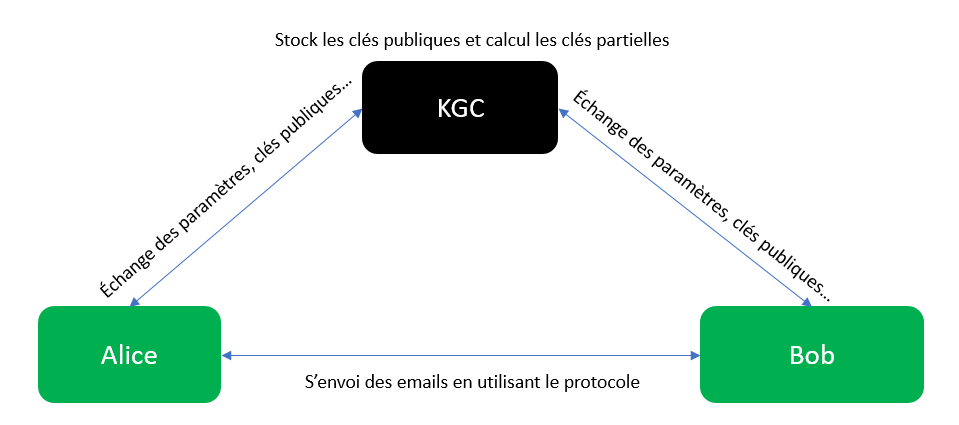
\includegraphics[width=14cm]{images/SchemaGlobal.png}
	\caption{Schéma global du protocole}
	\label{fig:globalProtocol}
\end{figure}
%TODO compléter ce chapitre et préciser les actions des acteurs plus en détails
\section{Acteurs}
Les parties impliquées sont les suivantes comme vu à la figure \ref{fig:globalProtocol}.
\begin{itemize}
	\item Alice : L'envoyeur du mail en direction de Bob. Alice doit discuter avec le KGC pour construire sa clé privée (afin de signer) et récupérer la clé publique de Bob.
	\item Bob : Le destinataire du message, communique uniquement avec le KGC en ayant reçu le message d'Alice afin de récupérer sa clé publique pour vérifier la signature et de construire sa clé privé pour déchiffrer le message.
	\item KGC : Permet aux différents acteurs de pouvoir récupérer les clés publiques des clients, mais aussi de  recevoir les \textit{Partial Private Keys} qui permettent aux acteurs de construire leur clé privée. 
\end{itemize}
Ces partis sont les principaux présents dans un exemple de \textit{Certificateless Cryptography} dans mon système de mail.
\section{Fonctionnement Certificateless PKC}
Je vais ici découper les différents algorithmes présent dans le certificateless public key cryptography. En passant par le chiffrement et la signature.
Ces algorithmes seront accompagnés d'explications sur leur utilité. Les noms donnés aux algorithmes seront réutilisés ensuite pour les schémas afin de démontrer l'architecture du protocole mis en place. L'on peut voir des définitions spécifiques dans l'article sur lequel je me suis appuyé pour ce travail~\cite{DBLP:conf/pkc/DentLP08}.
\subsection{Chiffrement}
Liste des différents algorithmes de \textit{Certificateless Cryptography} et leur description, les détails techniques de leurs implémentations sont disponibles à la Section \ref{sec:primitiveSearch}.
\begin{itemize}
	\item \textit{Setup.} (seulement une fois par le KGC).
	\item \textit{Partial-Private-Key-Extract.} Calcul d'une clé privée partielles lorsque qu'un client le demande pour identité donnée.
	\item \textit{Set-Secret-Value.} Le client ne le fait qu'une fois pour tirer sa valeur secrète.
	\item \textit{Set-Private-Key.} Le client combine ses clés partielles et sa clé secrète pour obtenir une clé privée afin de déchiffrer les message reçus, chiffrés avec une certaine identité.
	\item \textit{Set-Public-Key.} Le client ne le fait qu'une fois, il calcule sa clé publique en fonction de sa valeur secrète.
	\item \textit{Encrypt.} Chiffre un message avec la clé publique du destinataire et son identité.
	\item \textit{Decrypt.} Déchiffre un message utilisant sa clé privée et l'identité utilisée pendant le chiffrement.
\end{itemize}
\subsection{Signature}
Pour la signature les algorithmes sont les mêmes avec une différence dans leur conception et évidemment le \textit{Encrypt} et \textit{Decrypt} sont remplacé par \textit{Sign} et \textit{Verify}.
%TODO compléter voir tableau
Dans la littérature certificateless les schémas de signatures sont beaucoup plus cassés que ceux de chiffrement apparemment (voir tableau ). Il faut donc faire attention à suivre les schémas afin de vérifier que le schéma choisi ne soit pas mis à mal.
\section{Design du protocole}
%TODO : ajouter setup
\begin{figure}
[h!]
	\centering
	\begin{sequencediagram}
		\newthread{A}{Alice}{}
		\newinst[8]{B}{KGC}{} 
		\begin{call}{A}{Initialisation with alice@mail.ch}{B}{OK, $mpk_E, mpk_S$}
		\end{call}
	\postlevel
		\begin{callself}{A}{\shortstack{SetSec $x_E = Z_p^*$ \\ SetSecSig $x_S = Z_p^*$}}{}
		\end{callself}
	\postlevel
		\begin{callself}{A}{\shortstack{SetPub $PKE_{Alice} = (g^{x_E}, g_{1}^{x_E})$\\SetPubSig $PKS_{Alice} =x_SP$}}{}
		\end{callself}
	\postlevel
		\begin{call}{A}{$PKE_{Alice}, PKS_{Alice}$}{B}{}
		\end{call}
		
	\end{sequencediagram}
	\caption{Schéma de la première connexion}
	\label{fig:firstConn}
\end{figure}

Dans la Figure \ref{fig:firstConn} l'on voit la première connexion d'un utilisateur.
Alice veut s'enregistrer auprès du KGC, ainsi le KGC lui renvoi les paramètres publiques (mpkS et mpkE) si aucun utilisateur n'a déjà cet email. Ces paramètres publiques sont assez lourd, en effet, ils font environ 52 kB au total, c'est donc un gros paquet qui est envoyé là. Dans mes expérimentations je n'ai jamais eu de problèmes, mais il est préférable de le mentionner tout de même.
L'utilisateur va alors crée sa valeur secrète tirée aléatoire modulo p puis générer sa clé publique.
Pour finir Alice envoi sa clé publique au KGC afin qu'il l'associe à son ID et puisses le donner aux personnes qui veulent envoyer un mail à Alice.\\

%\begin{figure}[h!]
	%\centering
	%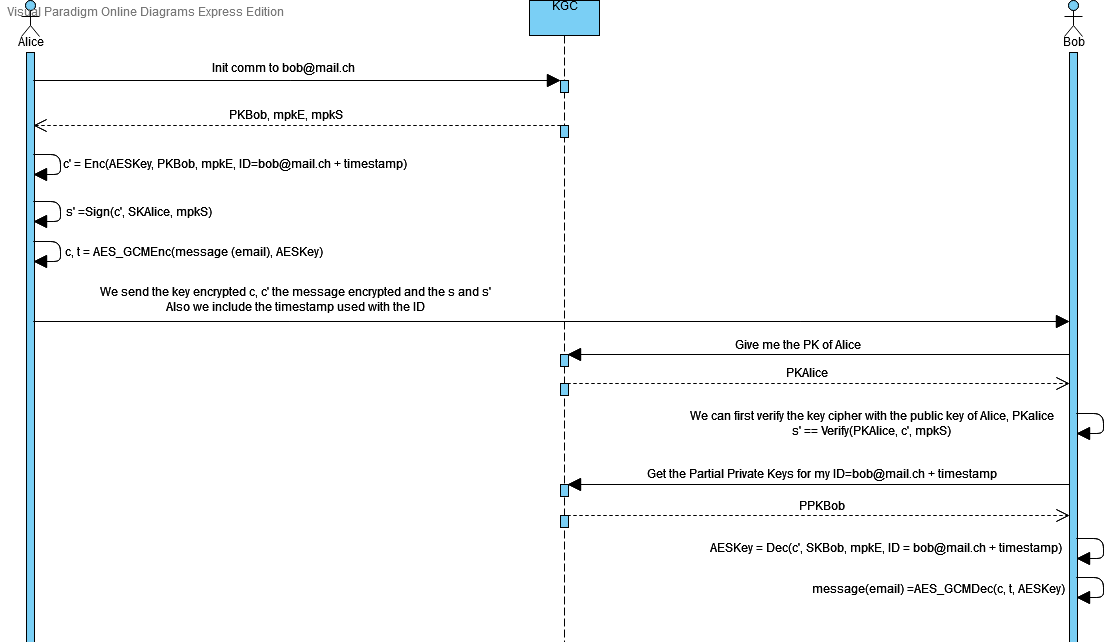
\includegraphics[width=14cm]{images/aliceSendsToBob.png}
	%\caption{Alice envoi un message à Bob}
	%\label{fig:aliceSends}
%\end{figure}

\begin{figure}[h!]
	\centering
	\begin{sequencediagram}
		\newthread{A}{Alice}{}
		\newinst[7]{B}{KGC}{} 
		\newinst[2]{C}{Bob}{}
		\begin{call}{A}{Comm. with bob@mail.ch}{B}{$PKE_{Bob} $}
		\end{call}
		\postlevel
		\begin{call}{A}{Extract alice@mail.ch + time}{B}{$PPKS_{Alice}$}
		\end{call}
		\postlevel
		\begin{callself}{A}{$c'  = ENC_{PKE_{Bob}}(AES_K, bob@mail.ch + time)$}{}
		\end{callself}
		\postlevel
		\begin{callself}{A}{SetPrivSig $SKS_{Alice} = (PPKS_{Alice}, x)$}{}
		\end{callself}
		\postlevel
		\begin{callself}{A}{$s' = Sign(c', SKS_{Alice})$}{}
		\end{callself}
		\postlevel
		\begin{callself}{A}{$c, t = AESGCM_{AESK}(mesage)$}{}
		\end{callself}
		\postlevel
		\begin{call}{A}{time, c', c, t, s', IV}{C}{}
		\end{call}
	\end{sequencediagram}
	\caption{Alice envoi un message à Bob}
	\label{fig:aliceSends}
\end{figure}

Dans la Figure \ref{fig:aliceSends} l'on voit comment se déroulerait l'envoi d'un message à Bob : 
\begin{itemize}
	\item Tout d'abord, Alice va récupérer le clé publique de Bob via son ID (aka email).
	\item Elle devra aussi récupérer sa clé privée partielle de signature pour créer ses clés privées afin de signer le message. Elle va le faire à l'aide de son ID et du même timestamp qu'utilisé pour la suite.
	\item Elle va ensuite tirer une valeur aléatoire dans Gt qui représentera sa clé AES pour la suite, elle va chiffrer cet élément à l'aide de la clé publique de Bob et de son ID complété par un timestamp. Ce timestamp sert à garder une certaine Forward Secrecy. Le cipher sera c'.
	\item Elle va calculer la signature du cipher donné (s' sur la figure)
	\item Alice utilisera un chiffrement authentifié comme AES\_GCM pour chiffrer et authentifié son mail à Bob, t pour le tag et c pour le cipher.
	\item Finalement elle va envoyer tout ces éléments à bob (à savoir, l'ID utilisé, c, c', t, s' et l'IV utilisé pour AES\_GCM).
\end{itemize}

\begin{figure}
[h!]
	\centering
	\begin{sequencediagram}
		\newthread{A}{Bob}{}
		\newinst[7]{B}{KGC}{} 
		\newinst[2]{C}{Alice}{}
		\begin{messcall}{C}{time, c', c, t, s', IV}{A}
		\end{messcall}
		\postlevel
		\begin{call}{A}{PK of alice@mail.ch}{B}{$PK_{Alice}$}
		\end{call}
		\postlevel
		\begin{callself}{A}{$s' == Verify(c', PK_{Alice})$}{}
		\end{callself}
		\postlevel
		\begin{call}{A}{Extract bob@mail.ch + time}{B}{$PPKE_{Bob}$}
		\end{call}
		\postlevel
		\begin{callself}{A}{SetPriv $SKE_{Bob}' = $}{}
		\end{callself}
		\postlevel
		\begin{callself}{A}{$AES_K = DEC_{SKE_{Bob}}(c', ID=bob@mail.ch+time)$}{}
		\end{callself}
		\postlevel
		\begin{callself}{A}{$message = AESGCM_{AES_K}(c,t, IV)$}{}
		\end{callself}
	\end{sequencediagram}
	\caption{Bob reçoit le message}
	\label{fig:bobReceives}
\end{figure}

Mais dans la Figure \ref{fig:bobReceives} l'on voit comment la réception du côté de Bob se déroulerait :
\begin{itemize}
	\item A la réception la première chose à faire et de vérifier le cipher de la clé AES. Pour cela l'on va demander la clé publique d'Alice au KGC. Puis on va vérifier ce cipher c' à l'aide de sa signature s'.
	\item Ensuite Bob va récupérer sa clé privée partielle via le KGC en fournissant son ID avec le timestamp envoyé par Alice. Il va ainsi pouvoir former sa clé privée.
	\item Avec s clé privée il va pouvoir déchiffrer c' et obtenir la clé AES pour la suite.
	\item Une fois que l'on a la clé AES l'on peut simplement déchiffrer à l'aide d'AES\_GCM c pour obtenir le message initial.
\end{itemize}


\chapter{Implémentation}
\label{ch:impl}
Ce chapitre présente le \textit{Proof Of Concept} mis en place pour prouver le bon fonctionnement du protocole proposé ainsi que d'évaluer son efficacité et sa simplicité d'utilisation. Les outils utilisés dans ce but sont présentés plus en détails en Annexe \ref{ch:outils}.
\section{Choix d'implémentations}
Cette section présente les différents choix d'implémentation faits au long du projet, afin d'avoir une idée globale du fonctionnement interne du POC.
\subsection{Langage}
Au départ le choix du langage s'est porté sur \textit{sagemath} (voir Annexe \ref{ch:outils}) afin de mieux comprendre les différents calculs et faire un premier POC du chiffrement/déchiffrement.
Cependant, l'implémentation du POC était lente et le changement d'algorithme pour les pairings était difficile.
Je me suis donc orienté sur le C pour avoir de meilleures performances et pouvoir mieux gérer la mémoire de mon implémentation. Pour pouvoir faire facilement des calculs sur les courbes elliptiques et les pairings en C il me fallait une librairie, ce que je décris dans la section suivante.

Comme on peut le voir sur la table \ref{table:comparisonTimeAlgo}, une différence des temps d'exécution entre les deux langages est bien réelle. Il faut cependant mettre en lumière que les temps sont calculés avec des courbes différentes et des couplages différents (Sage avec des Weil pairings, C avec des optimal ate pairings). Les résultats sont des moyennes faites sur 15 essais. Ils ont été effectués avec un processeur \textit{Intel(R) Core(TM) i7-7600U CPU @ 2.80GHz} et 16GB de RAM.

\begin{table}[h!]
	\centering
	\begin{tabular}{ |p{3cm}||p{3cm}|p{3cm}| }
		\hline
		\multicolumn{3}{|c|}{Temps des algorithmes entre les différents langages [s]} \\
		\hline
		Algorithmes & C & Sage\\
		\hline
		Setup   & 0.2856898 & 6.5858234\\
		Encrypt & 0.0061584 & 7.6450206\\
		Decrypt & 0.00951 & 3.3274426\\
		\hline
	\end{tabular}
\caption{Table de comparaison des temps d'exécution pour les différents algorithmes de Certificateless Cryptography }
\label{table:comparisonTimeAlgo}
\end{table}

\subsection{Librairie cryptographique}
En lisant le livre \textit{Guide to Paring-Based Cryptography}~\cite{bookPairing}, des librairies et implémentations en Sage sont conseillées et des exemples de codes sont montrés. C'est de ce livre que les recherches pour les différentes librairies ont commencées.

La librairie finalement utilisée est RELIC Toolkit~\cite{relic-toolkit} et en Annexe \ref{ch:outils}, c'est une librairie en cours de développement qui se veut efficiente. Sa concurrence avec MIRACL m'a fait hésiter dans mon choix, mais MIRACL est plus codée en C++ avec des équivalences en C, j'ai donc choisi RELIC. De plus j'ai trouvé que RELIC était généralement plus adapté dans le domaine universitaire pour des POC, puis il est plus efficient que d'autres librairies~\cite{performanceRELIC}.

\subsection{Courbe utilisée}
La courbe utilisée pour le POC est la BLS12-P381. Cette courbe est assez efficiente et compatible avec les pairings. De plus, RELIC l'a dans ses options et fonctionne bien, elle a un niveau de sécurité de 128bits. Je voulais prendre une courbe avec une plus grande sécurité, cependant RELIC ne l'a pas encore totalement implémentée (certains tests concernant $\mathbb{G}_2$ ne passent pas), mais la librairie étant toujours en cours de développement, il faudrait vérifier régulièrement pour pouvoir mettre la courbe à jour. Pour que RELIC utilise cette courbe il faut le mentionner à la compilation. Heureusement, la librairie établi des \textit{presets} pour la compilation de la librairie, la version GMP a été utilisée pour ce POC.

\subsection{Dérivation de la clé AES}
Le but du schéma certificateless est de chiffrer puis signer une clé AES qui permettra à mon message d'avoir un chiffrement authentifié. Pour cela il me faut dériver un élément de $\mathbb{G}_t$ en clé AES. En effet, le chiffrement dans le schéma certificateless se fait sur un élément de $\mathbb{G}_t$ et c'est donc plus simple de garder cet élément intact.

Pour cela j'ai utilisé une fonction permettant d'écrire sous forme compressée cet élément en bytes (fourni par la librairie RELIC utilisée et la fonction gt\_write\_bin()). Puis j'ai effectué un hachage avec SHA256 dessus, ainsi le résultat du hachage est une clé de 256 bits utilisable comme une \textit{master-key} pour une KDF. L'utilisation d'une KDF est toujours plus propre afin de créer au final une clé AES-256-GCM sûre. Pour la KDF la librairie libsodium (voir Annexe \ref{ch:outils}) a été utilisée.

\begin{sourcebox}{c}{Création de la clé AES depuis un élément $\mathbb{G}_T$}
	void get_key(char *aesk, gt_t originalM) {
		// Get the binary data of the Gt element
		int sizeAESK = gt_size_bin(originalM,1);
		uint8_t aeskBin[sizeAESK];
		gt_write_bin(aeskBin, sizeAESK, originalM, 1);
		uint8_t master_key[32];
		// Hash with SHA-256 to have an master key for KDF from the Gt binary data
		md_map_sh256(master_key, aeskBin, sizeAESK);
		// KDF the "master key" to have a usable key to encrypt the data
		crypto_kdf_derive_from_key(aesk, 32, 1, "AES-KEY", master_key);
	}
\end{sourcebox}

\subsection{Pseudo Forward Secrecy - Timestamp}
Afin d'obtenir une \textit{Pseudo Forward Secrecy} l'utilisation d'un timestamp dans l'ID est utilisée comme démontré dans la Section \ref{subsec:pseudoSecrecy}.

L'implémentation prend un timestamp par semaine, ainsi si une clé privé fuite, on ne pourra déchiffrer que les messages de cette semaine. Pour le lier à l'ID un "+" a été ajouté entre l'ID et le timestamp.
\begin{sourcebox}{C}{Gestion du timestamp}
	strcat(destinationTimestamp, "+");
	time_t timestampNow = time(NULL);
	// Calcul afin d'avoir un timestamp par semaine
	timestampNow -= timestampNow % SECONDS_IN_WEEK;
	sprintf(timestampStr, "%d", timestampNow);
\end{sourcebox}

\subsection{Fonctions de hachage - signature}
Pour le schéma de signature, il nous faut plusieurs fonctions de hachage différentes. En effet, ce schéma est basé sur le \textit{Random Oracle Model} comme défini dans le Chapitre \ref{ch:analysis}. Pour appliquer cela, j'ai utilisé la même méthode de mapping disponible dans RELIC pour mapper une char array (tableau de byte) à un point sur G2 à savoir g2\_map.
Pour H1, la première fonction de hachage, j'ai simplement utilisé cette fonction directement, mais pour H2 et H3 j'ai ajouté un byte devant les données à mapper, respectivement les bytes '01' et '02'. Ceci afin de séparer les domaines des résultats des hashs, cela s'appelle du \textit{Hash Domain Separation}. En effet, on peut voir que ce draft~\cite{irtf-cfrg-hash-to-curve} défini cela comme une simulation pour prendre en compte plusieurs \textit{Random Oracle}.

\begin{sourcebox}{c}{Fonction H2 pour le hachage vers un point de la courbe $\mathbb{G}_2$}
	void functionH2(g2_t* to_point, char* bytes_from, int len_bytes){
		uint8_t to_hash[len_bytes + 1];
		// Hash domain separation adding 1 byte \x01 before the actual data to hash
		to_hash[0] = '\x01';
		memcpy(to_hash + 1, bytes_from, len_bytes);
		g2_map(*to_point, to_hash, len_bytes + 1);
	}
\end{sourcebox}

\subsection{Sérialisation des données}
Pour la sérialisation des données, typiquement les clés publiques et les clés privées partielles envoyées en réseau ou les clés publiques enregistrées dans les fichiers par exemple, j'ai utilisé la librairie binn (voir Annexe~\ref{ch:outils}). Cela permet de "packer" facilement des données binaires, pour cela RELIC met à disposition des méthodes g1\_write\_bin g1\_read\_bin qui a permis de faire ces enregistrements binaires. Ainsi les transferts de données sont simplifiés.

Cependant, il faut faire attention à certaines choses, on ne peut lire et écrire simultanément à l'aide de binn, si l'on crée un objet via un buffer on ne pourra pas modifier cet objet. Cela m'a posé des problèmes pour l'enregistrement des données secrètes, j'ai donc dû copier l'objet lu pour pouvoir le modifier et sauver les nouveaux paramètres.

\subsection{Enregistrement des clés publiques (serveur)}
Pour l'enregistrement j'ai utilisé une petite base de données NoSQL stockant les clés publiques des utilisateurs sur le KGC. Cela permet de facilement récupérer une clé publique pour un utilisateur si besoin. Pour implémenter cela j'ai utilisé la librairie UnQlite (voir Annexe~\ref{ch:outils}). J'ai stocké les clés publiques pour le schéma de signature et de chiffrement séparément. En effet, l'entrée pour la signature porte le nom "signature/ID" et le chiffrement "encryption/ID".

\subsection{Récupération via IMAP}
Utilisation de la librairie libetPan (voir Annexe~\ref{ch:outils}) et de l'exemple \textit{imap-sample.c} pour la récupération email par IMAP. IMAP a été choisi plutôt que POP3 afin de laisser les messages sur le serveur et ainsi avoir plusieurs appareils pouvant y accéder. Pour parser les emails cette librairie est aussi choisie ainsi que son exemple \textit{mime-parse.c}.

\section{Implémentation clés  de chiffrement}
Pour pouvoir implémenter ce schéma de chiffrement et signature certificateless dans un système hybride, il a fallu penser à une manière d'encapsuler la clé et les données. Pour cela j'ai essayé de faire un système comparable à la Figure \ref{fig:encapsulate}.

\begin{figure}[h!]
	\centering
	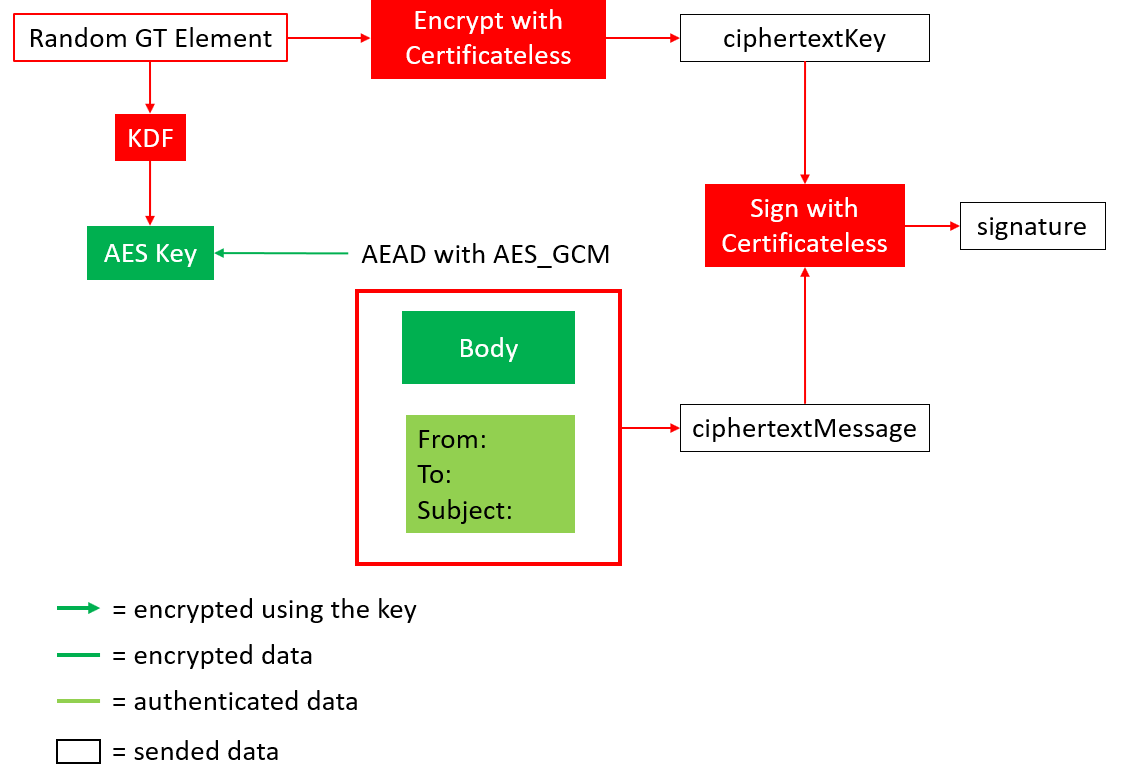
\includegraphics[width=\textwidth]{images/schemCles.png}
	\caption{Schéma encapsulation des données}
	\label{fig:encapsulate}
\end{figure}

\section{Fonctionnement global POC (KGC)}
Présentation du fonctionnement global de l'implémentation du KGC pour le POC. De plus, les problèmes connus et des propositions d'améliorations sont présentés.
\subsection{Fonctionnement}
Le KGC est un élément important du protocole, en effet c'est lui qui va fournir une partie de la clé privée de l'utilisateur. Dans ce cas, il permet de distribuer les clés publiques de ses utilisateurs, mais habituellement on fera plutôt appel à un serveur dédié pour la gestion des clés.

Par mesure de généricité j'ai établi des codes d'opérations (arbitraires) afin de définir les opérations demandées au serveur par le client. Cela à l'aide de la librairie binn et les constructions d'objets proposés.

\paragraph*{Structure des paquets reçus.}
Pour la structure des paquets que le KGC va traiter, ils se présentent sous la forme d'un objet binn qui a comme propriétés au moins un code d'opération \textbf{opCode} et un \textbf{ID} associé. Cela permet de trier le paquet et de l'associer à une opération afin de traiter la donnée amenée avec le paquet. L'ID sert aussi différemment en fonction des codes employés.

Ainsi un paquet typique sera :\\
\{opCode: PK, ID : alice@wonderland.com, payload : xxx\}
\paragraph*{Codes d'opérations.}
Les différents codes d'opérations sont :
\begin{itemize}
	\item HELO : Permet de s'annoncer au KGC pour la première fois, le KGC répondra systématiquement avec les paramètres globaux du système. Cela implique la Master Public Key de chiffrement du KGC ainsi que celle du schéma de signature. 
	\item PK : Permet d'annoncer les clés publiques de l'utilisateur avec un certain ID. Le paquet est composé de \{ID : alice@wonderland.com, opCode : PK, PKE : base64 de la PKE, PKS : base64 de la PKS\}. La PKE est encodée en base64 par le client puis est envoyée au serveur. Elle est aussi représentée à l'aide d'un objet binn mais le serveur n'a pas besoin d'en prendre connaissance, il stocke donc cette donnée telle quelle dans la base de donnée NoSQL. La même chose est faite pour la PKS, la clé publique pour la signature.
	\item GPE : Permet de récupérer la clé publique de chiffrement (utile pour chiffrer un message) d'un utilisateur ayant l'ID mentionné. Ainsi le serveur va simplement regarder dans la base de donnée pour "encryption/ID" et récupérer la clé encodée en base64 et la renvoyer à l'utilisateur. Si le serveur ne trouve pas cette clé, il va renvoyer une erreur dans l'objet et ainsi à la réception on va d'abord regarder cette erreur.
	\item GPS : Fonctionne de la même manière que "GPE" mais pour les clés publiques de Signature (utile pour vérifier une signature).
	\item SE : Permet de faire la "Signature Extraction" et donc de demander la Partial Private Key pour l'utilisateur ID. Utilisé lors de la signature d'un message afin de construire sa clé privée et de signer le message avec. 
	\item EE : Permet de faire la "Encryption Extraction" et donc de demander la Partial Private Key pour l'utilisateur ID. Utilisé lors du déchiffrement d'un message pour reconstruire sa clé privée.
\end{itemize}
\subsection{Problème rencontré}
Un problème ayant bien ralenti le développement est une erreur dans l'implémentation des socket en C. En effet, au départ le serveur ne recevait pas toutes les données du client et inversement d'ailleurs.

La solution a été de recevoir les données par petits chunks et de les regrouper petit à petit. Beaucoup de tests et de recherches ont été faites pour ce problème pourtant anodin sur les socket en C.
\subsection{Problèmes connus}
Liste des problèmes connus concernant l'implémentation du côté serveur.
\paragraph*{Implémentations TLS}
Pour avoir une sécurité supplémentaire et garantir l'authenticité des paramètres envoyés par le KGC il serait préférable d'implémenter les serveur en TLS. Ceci n'a pas été fait dans l'état actuel du projet.
\paragraph*{Sauvegarde des paramètres}
La sauvegarde des paramètres privés du serveur n'est pas implémentée dans le KGC actuellement ce qui amènerait des problèmes lors d'un crash ou un arrêt du serveur. Ceci doit être résolu dans une implémentation effective.
\paragraph*{Révocation des clés}
La révocation des clés n'est pas réellement implémentée, dans l'état actuel le serveur va reprendre une nouvelle clé publique envoyée d'Alice car aucune vérification n'est faite, ceci permet de révoquer une clé en l'écrasant. Cependant ce n'est pas une vrai révocation de clés.
\subsection{Améliorations}
Quelques améliorations seraient possibles mais restent à mettre en place, cela permet de donner quelques pistes pour la continuation du travail :
\paragraph*{Vérification email.}
Implémentation d'une vérification par email afin d'être sûr que l'adresse email annoncée appartient bien à l'utilisateur qui s'authentifie pour la première fois. Typiquement lors du "HELO", on pourrait envoyer un mail de vérification avec un code sur l'email annoncé (s'il n'est pas dans la base de données) et demander le code envoyé avant de pouvoir uploader sa clé publique. Ainsi le client devrait pouvoir implémenter cette fonctionnalité aussi. Cela permettrait d'être sûr que tel utilisateur a effectivement tel email.
\paragraph*{Mise en place à large échelle}
Si l'on veut pouvoir mettre en place ce genre de système à une large échelle, il faut prévoir une manière d'avoir plusieurs KGC qui communiquent, par exemple, entres eux dans un système global de réplication. Ceci afin de pouvoir avoir les mêmes paramètres sur l'ensemble des KGC et que le système fonctionne.

Une autre solution serait par exemple d'ajouter un "tag" d'appartenance à un ID et celui-ci sera donc lié à un certain KGC. Ceci afin de partager la charge qui serait normalement sur un seul KGC. Ce genre de solutions pourrait permettre d'avoir par exemple un KGC par domaine ou alors de les partager via les TLDs. De plus, les KGC pourraient avoir des paramètres générés différemment entre eux, ce qui ne serait pas le cas dans un système de réplication. Cette solution ajoute cependant de la complexité au système. Et des envoi de paquets plus volumineux sur le réseau pour les paramètres globaux d'un KGC qui sont de 52kB, pour chaque KGC.

Pour le système de clés on pourrait reprendre l'idée de~\cite{journals/ijnsec/BalakrishnanR16} afin d'aller chercher le serveur de clés pour tel domaine.
\section{Fonctionnement global POC (Client)}
Présentation du fonctionnement global de l'implémentation du client mail implémentant la CLPKC pour le POC, des améliorations possibles et des problèmes connus.
\subsection{Fonctionnement}
Le déroulement pour envoyer un message se passe comme suit :
\begin{itemize}
	\item Informations de connexions à GMail demandées
	\item Si le fichier (\textit{globalMPK}) de paramètres globaux n'est pas présent en local l'application communiquera avec le KGC afin de récupérer ces paramètres publiques tels que $mpk_E$ et $mpk_S$ et les stockera donc.
	\item Si le fichier (\textit{ID\_SK}) n'est pas trouvé les valeurs secrètes vont être tirées pour l'utilisateur et la construction des clés publiques et leur envoi au serveur va être effectué. Si le fichier est trouvé il va être déchiffrer en utilisant AES\_GCM en prenant la clé donnée par l'application de l'algorithme Argon2id sur un mot de passe donné par l'utilisateur.
	\item L'application va demander si l'utilisateur veut envoyer ou recevoir des emails.
	\item Dans le cadre d'un envoi, les informations nécessaires à l'envoi d'un mail seront demandées telles que le destinataire, le sujet et le message.
	\item L'application va regarder si le fichier \textit{ID\_PK} est disponible en local et si ce n'est pas le cas il va demander au KGC la clé publique du destinataire. Si le KGC n'arrives pas à la trouver une erreur sera annoncée à l'utilisateur et l'envoi ne sera pas effectué.
	\item Si tout est bon l'application va effectuer l'encapsulation des données montrées dans la Figure \ref{fig:encapsulate}.
	\item L'envoi est effectué via SMTP en incluant dans les headers le base64 des informations nécessaires à la réception.
	\item Les informations confidentielles sont sauvegardées en les chiffrant à l'aide AES\_GCM et Argon2id afin de dériver le mot de passe de l'utilisateur.
\end{itemize}
La réception se passe de la même manière globalement, le changement principal et le téléchargement des emails des dernières 24h grâce à IMAP, à moins qu'ils soient déjà téléchargés auparavant. Le déchiffrement va se passer comme décrit dans le Chapitre \ref{ch:arch}. 
\subsection{Fonctionnalités}
\paragraph*{Sécurité connexion mail.}
Pour la connexion au serveur SMTP / IMAP j'ai fait attention à la connexion sécurisée pour éviter de \textit{leak} des mots de passe des utilisateurs du POC. En effet, cela permet de chiffrer les communications avec les serveurs de Gmail comme démontré dans la Figure \ref{fig:securityProofEmail}.
\begin{figure}[h!]
	\centering
	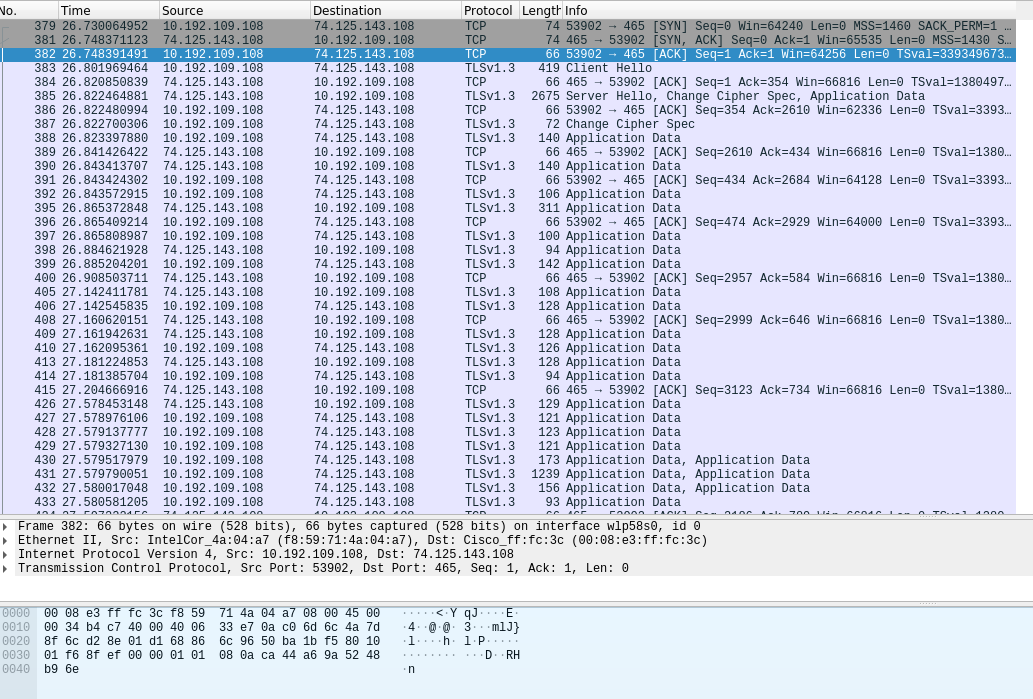
\includegraphics[width=14cm]{images/packetProofEncrypted.png}
	\caption{Connexion SSL/TLS avec le serveur email}
	\label{fig:securityProofEmail}
\end{figure}
\subsection{Problèmes connus}
Les problèmes qu'il reste à résoudre à ce jour :
\paragraph*{Développement sécurisé.}
Lors du développement j'ai fait attention au maximum d'avoir le moins possible de fuites mémoires à l'aide de sanitizers et de valgrind. Cependant cela ne suffirait pas pour une application correctement sécurisée, il faudrait mettre à 0 les structures utilisées et qui stockent des informations confidentielles.
\paragraph*{Enregistrement lors d'un crash}
Lors d'un crash du client en plein milieu du programme ou de l'écriture/chiffrement du fichier des secrets il se peut que celui-ci deviennent corrompu. Il faudrait éviter de le corrompre car la seule manière d'y remédier serait de le supprimer et ainsi de recréer ses valeurs secrètes.
\subsection{Améliorations}
Les améliorations à amener dans le client :
\paragraph*{Multiples destinataires.}
Pour le moment l'implémentation ne prends pas en compte une situation où un mail doit être envoyé à des destinataires multiples, c'est une fonctionnalité importante à mettre en œuvre dans une implémentation de client mail. Pour ce faire, il faudra spécifier dans les headers l'utilisateur ciblé par tel cipher et signature. Ainsi, lors de la réception, le client prendra les options X-ID-CIPHER-B64 p.ex. Ou alors trouver un moyen d'envoyer un mail différent à chaque utilisateur, sans perdre la possibilité qu'un destinataire puisse choisir de répondre à tous les autres destinataires.
\paragraph*{Possibilité d'ajouter des pièces jointes.}
Pour le moment la possibilité d'ajout de pièces jointes n'a pas été pris en considération. Cependant, une des librairies choisies pour la réception des mails pourrait composer des messages contenant des pièces jointes. Il faudrait ainsi les chiffrer avec la clé symétrique avant de l'ajouter dans le mail.
\paragraph*{GUI.}
Mettre en place une interface utilisateur pour le client mail, cela aiderait à rendre le chiffrement plus transparent et plus simple pour l'utilisateur. En effet, demander à l'utilisateur d'écrire son mail au terminal n'est pas spécialement agréable.
\paragraph*{Ajout clé publique}
Dans l'envoi du mail il faudrait ajouter la clé publique de la source dans le message, ainsi que la vérification de la signature.

\paragraph*{Répudiation et non répudiation}
Ajouter la possibilité de signer ou non l'email afin de pouvoir obtenir ou non de la répudiation. Pour le moment l'implémentation signe le message et la clé symétrique chiffrée, ainsi la non-répudiation est accomplie. Afin d'avoir de la non répudiation il faudrait ne plus avoir cette signature, cela permettrait d'avoir la répudiation et d'avoir tout de même un système sécurisé.

\section{Comparaisons avec l'état de l'art}
Dans cette section je vais présenter les différents protocoles et implémentations existantes présentées au Chapitre \ref{ch:analysis} et les comparer à l'implémentation faite dans ce travail (ci-après CLPKC-POC). Tout d'abord en présentant les différentes propriétés cryptographiques, les tailles d'overhead et l'utilisabilité.

\subsection{Propriétés cryptographiques}
Ici je fais un comparatif sur les différentes propriétés cryptographiques que les systèmes de mails sécurisés proposent avec mon implémentation Certificateless. On peut le voir dans la table \ref{table:comparisonProperties}. La pseudo forward secrecy est intéressante mais expliquée dans la Section \ref{subsec:pseudoSecrecy}. La répudiation est une propriété possible dans CLPKC en évitant de signer la clé symétrique chiffrée. La non répudiation est établie via les signatures digitales des différents algorithmes, dans CLPKC POC la signature se fait sur le message chiffré et la clé chiffrée ainsi la source ne pourra répudier le fait d'avoir signer ces données. 
\begin{table}[h!]
	\centering
	\begin{tabular}{ |p{3cm}||p{3cm}|p{3cm}|p{3cm}| }
		\hline
		\multicolumn{4}{|c|}{Comparaisons des propriétés cryptographiques proposées} \\
		\hline
		Propriétés & CL-PKC POC & PGP & S/MIME \\
		\hline
		E2EE   & Oui & Oui & Oui\\
		Forward Secrecy & Oui (Pseudo) & Non & Non\\
		Repudiation & Possible & Non & Non\\
		Non repudiation & Oui & Oui & Oui\\
		\hline
	\end{tabular}
	\caption{Table de comparaison des différentes propriétés cryptographiques }
	\label{table:comparisonProperties}
\end{table}
\subsection{Overhead induit}
Ici je présente les différents \textit{overhead} que j'ai remarqué en utilisant les différents systèmes de mails sécurisés analysés au Chapitre \ref{ch:analysis}. Dans le tableau \ref{table:comparisonOverhead} on voit la taille d'overhead induit par les différents systèmes testés. Ces tailles ont été déterminées de manière empirique par des tests effectués tout au long de ce projet.
\begin{table}[h!]
	\centering
	\begin{tabular}{ |p{3cm}||p{4cm}|p{6cm}| }
		\hline
		\multicolumn{3}{|c|}{Comparaisons de l'overhead induit dans un mail} \\
		\hline
		Implémentations & Taille overhead & Contenu\\
		\hline
		CLPKC-POC   & Environ 1000 bytes / destinataire & Signature, timestamp, nonce, Encrypted Session Key\\
		PGP & Environ 300 bytes / destinataire & Encrypted Session key\\
		S/MIME & Environ 7300 bytes (Signature) & CMS EnvelopedData et Certificat\\
		\hline
	\end{tabular}
	\caption{Table de comparaison des différents overhead en rapport avec les solutions existantes }
	\label{table:comparisonOverhead}
\end{table}

\subsection{Différences d'utilisabilité}
Comparaison de la facilité d'utilisation entre PGP, S/MIME et CLPKC-POC. Cela permet de comparer les différents cas d'utilisation et de voir la souplesse des différentes solutions.

\paragraph*{Usage global}
Globalement l'utilisation de CLPKC-POC est souvent plus simple que l'utilisation de PGP ou S/MIME. En fait, l'utilisation sera plus simple car le système de cryptographie \textit{Certificateless} a certaines propriétés qui le rend plus accessible. 

Dans S/MIME le contrôle des certificats et l'import de différents certificats est complexe et peut entrainer des erreurs. Dans PGP les clés ne sont pas si faciles à obtenir et les clés nécessitent aussi d'avoir une certaine confiance (signés par d'autres utilisateurs) de PGP.
\paragraph*{KGC / serveurs de clés non accessibles}
Que se passe-t-il si un serveur de clés ou le KGC n'est plus accessible pour une quelconque raison ?

Dans le cas de PGP, le déchiffrement pourra être effectué car la clé privée ne change pas d'un moment à l'autre. De plus, lors d'un chiffrement PGP la signature digitale est effectuée sur le texte clair puis est chiffrée avec. Ainsi la clé publique de la source doit être récupérée, cela posera un problème si la clé n'est pas déjà stockée en local. Dans certains cas la clé publique peut être intégrée à l'envoi dans l'email mais n'est pas authentifiée.

Dans le cas de CLPKC-POC, le déchiffrement sera potentiellement compromis, cela dépendra si l'utilisateur aura créé la clé pour la semaine courante ou non. Si c'est le cas, le chiffrement pourra être fait. La vérification de la signature pourra être faite aussi si la clé publique de la source est stockée en local (si l'utilisateur nous a envoyé un mail auparavant). Il serait possible d'envoyer la clé publique de la source pour faciliter la vérification mais ce n'est pas fait dans l'état actuel.

Dans S/MIME, le déchiffrement pourra être effectué car la clé privée ne changera pas non plus. La vérification pourra être faite en local avec les CAs intégrés dans le système pour le certificat envoyé avec le mail.
\paragraph*{Erreur utilisateur}
Les erreurs que les utilisateurs peuvent faire sur certains éléments peuvent être problématiques dans certains cas pour PGP et S/MIME. En effet, si un utilisateur signe une clé publique d'un utilisateur sans vérifier réellement l'identité cela pourrait authentifier une clé publique compromise et déstabiliserait le \textit{Web Of Trust}.

 Pareil pour S/MIME où l'import d'un certificat malicieux pourrait avoir un impact sur la sécurité des données. Cependant, dans CLPKC-POC peu d'erreurs peuvent être faites car la plupart des paramètres et clés sont générés automatiquement.

\chapter{Conclusion}
\label{ch:conclusion}
Lors de ce travail de bachelor la problématique principale 
\pagebreak

% +---------------------------------------------------------------+
\cleardoublepage
\addcontentsline{toc}{chapter}{Bibliographie}
\renewcommand{\thechapter}{}
\renewcommand{\chaptername}{}
\chaptermark{Bibliographie}
\bibliographystyle{plain}
\bibliography{chapters/biblio}
\nocite{*} %ajoute tout ce qu'il y a dans le bibtex
\cleardoublepage
\chaptermark{Liste des Figures}
\listoffigures
\cleardoublepage
\chaptermark{Liste des tableaux}
\listoftables

% Annexes
% +---------------------------------------------------------------+
\appendix

\chapter{Outils utilisés pour la compilation}

\section{RELIC Toolkit}
Pour pouvoir faire des calculs de \textit{Pairings} et sur des courbes elliptiques je me suis fier à RELIC Toolkit~\cite{relic-toolkit} qui est une librairie C permettant ce genre de calculs assez simplement.\\
Cette librairie demande à être compilée avec une certaine courbe et certaines options (typiquement fonction de hachage et autres...). Des presets existent et c'est donc ce que j'ai utilisé pour ce POC. Cela demande donc de fournir la librairie précompilée avec les bonnes options pour l'utilisateur. L'inconvénient c'est donc que pour mettre à jour une courbe il va falloir recompiler toute la librairie et la fournir à l'utilisateur, néanmoins on n'aura pas à changer de code.

\section{Libsodium}
Pour faire du chiffrement authentifié j'ai utilisé libsodium\footnote{https://libsodium.gitbook.io/doc/}, en effet, m'étant un peu familiarisé avec la librairie il m'a semblé être le choix le plus évident en plus de fournir des méthodes de chiffrement simples à mettre en place. Nécessite d'avoir libsodium en librairie linkée.

\chapter{Fichiers}
\label{ch:fichiers}
Liste des fichiers annexes au rapport, ce qu'ils contiennent et comment les utiliser si besoin.
\section{Code du \textit{Proof Of Concept}}
Le code est en annexe du rapport avec le nom \textit{POCCertificateless}.
Le \textit{README.md} présent à la source devrait être suffisant pour compiler soi-même le code. De plus, un repository github contenant le code, testé sur une installation Ubuntu 20.04 est disponible à l'adresse \url{https://github.com/mbonjour/POCCertificateless}.

Le code est commenté à la manière \textit{Doxygen} afin d'avoir des informations à chaque fois qu'une fonction est référencée. De plus, le code est commenté afin de comprendre le déroulement global des différentes parties. Le code va générer ainsi trois exécutables dont le client, le serveur et un test afin de calculer le temps mis par les algorithmes et utilisé anciennement pour se représenter le déroulement global d'un échange entre Alice et Bob.
\section{Tableaux comparatifs}
Les tableaux comparatifs cités dans le chapitre \ref{ch:analysis} apparaissent sous forme de feuille dans un fichier excel se nommant \textit{ComparatifsCLPKCSchemes.xlsx}. 
La feuille nommée CLEs contient un comparatif des schémas de chiffrement tandis que la feuille CLSs contient un comparatif des schémas de signatures.

Ces tableaux sont mis en annexes car il représente une grande quantité de données qui apparaissait mal dans ce rapport.


\end{document}
